\documentclass[a4paper]{article}
\usepackage[spanish]{babel}
\usepackage[utf8]{inputenc}
\usepackage{charter}   % tipografia
\usepackage{graphicx}
\usepackage{enumerate}
\usepackage{listings}
\usepackage{color}
%\usepackage{indentfirst}
\usepackage{fancyhdr}
\usepackage{latexsym}
\usepackage{lastpage}
\usepackage[colorlinks=true, linkcolor=black]{hyperref}
%\usepackage{makeidx}
%\usepackage{float}
\usepackage{calc}
\usepackage{amsthm, amssymb}
\usepackage[nosumlimits]{amsmath} % este package hace que se vean mal los incides en las sumatorias, pero permite poner uno abajo del otro en la ecuacon de los L de laagrange

\usepackage{subfig}

\usepackage{amsfonts}

%\usepackage{sectsty}
%\usepackage{charter}
%\usepackage{wrapfig}
%\usepackage{listings}
%\lstset{language=C}
\definecolor{gray}{gray}{0.5}
\definecolor{light-gray}{gray}{0.95}
\definecolor{orange}{rgb}{1,0.5,0}

\usepackage{color} % para snipets de codigo coloreados
\usepackage{fancybox}  % para el sbox de los snipets de codigo

\definecolor{litegrey}{gray}{0.94}

% \newenvironment{sidebar}{%
% 	\begin{Sbox}\begin{minipage}{.85\textwidth}}%
% 	{\end{minipage}\end{Sbox}%
% 		\begin{center}\setlength{\fboxsep}{6pt}%
% 		\shadowbox{\TheSbox}\end{center}}
% \newenvironment{warning}{%
% 	\begin{Sbox}\begin{minipage}{.85\textwidth}\sffamily\lite\small\RaggedRight}%
% 	{\end{minipage}\end{Sbox}%
% 		\begin{center}\setlength{\fboxsep}{6pt}%
% 		\colorbox{litegrey}{\TheSbox}\end{center}}

\newenvironment{codesnippet}{%
	\begin{Sbox}\begin{minipage}{\textwidth}\sffamily\small}%
	{\end{minipage}\end{Sbox}%
		\begin{center}%
		\colorbox{litegrey}{\TheSbox}\end{center}}



\usepackage{fancyhdr}
\pagestyle{fancy}

%\renewcommand{\chaptermark}[1]{\markboth{#1}{}}
\renewcommand{\sectionmark}[1]{\markright{\thesection\ - #1}}

\fancyhf{}

\fancyhead[LO]{Sección \rightmark} % \thesection\ 
\fancyfoot[LO]{\small{nombre, nombre, nombre}}
\fancyfoot[RO]{\thepage}
\renewcommand{\headrulewidth}{0.5pt}
\renewcommand{\footrulewidth}{0.5pt}
\setlength{\hoffset}{-0.8in}
\setlength{\textwidth}{16cm}
%\setlength{\hoffset}{-1.1cm}
%\setlength{\textwidth}{16cm}
\setlength{\headsep}{0.5cm}
\setlength{\textheight}{25cm}
\setlength{\voffset}{-0.7in}
\setlength{\headwidth}{\textwidth}
\setlength{\headheight}{13.1pt}

\renewcommand{\baselinestretch}{1.1}  % line spacing


% \setcounter{secnumdepth}{2}
\usepackage{underscore}
\usepackage{caratulaV}
\usepackage{url}
\usepackage{float}

%\usepackage{makeidx}


% \setcounter{secnumdepth}{2}
\usepackage{underscore}
\usepackage{alltt}
\usepackage{tikz}
\usepackage{color}
% \usepackage{gnuplottex}
\usepackage{verbatim}
\usepackage{algorithm}
\usepackage{algpseudocode}

\definecolor{dkgreen}{rgb}{0,0.6,0}
\definecolor{gray}{rgb}{0.5,0.5,0.5}
\definecolor{mauve}{rgb}{0.58,0,0.82}

\lstset{frame=tb,
  language=Python,
  aboveskip=3mm,
  belowskip=3mm,
  showstringspaces=false,
  columns=flexible,
  basicstyle={\small\ttfamily},
  keywordstyle=\color{blue},
  commentstyle=\color{dkgreen},
  stringstyle=\color{mauve},
  breaklines=true,
  breakatwhitespace=true,
  tabsize=3,
  numbers=left,
  xleftmargin=2em,
  frame=single,
  framexleftmargin=2em,
  numbersep=5pt,                   % how far the line-numbers are from the code
  numberstyle=\small\color{gray} % the style that is used for the line-numbers
 }

\parskip = 5 pt

\newcounter{row}
\newcounter{col}

\newcommand\setrow[3]{
	\setcounter{col}{1}
	\foreach \n in {#1, #2, #3} {
	\edef\x{\value{col} - 0.5}
	\edef\y{3.5 - \value{row}}
	\node[anchor=center] at (\x, \y) {\n};
	\stepcounter{col}
	}
	\stepcounter{row}
}



\newcommand\setrowaux[7]{
	\setcounter{col}{1}
	\foreach \n in {#1, #2, #3, #4, #5, #6, #7} {
	\edef\x{\value{col} - 0.5}
	\edef\y{7.5 - \value{row}}
	\node[anchor=center] at (\x, \y) {\n};
	\stepcounter{col}
	}
	\stepcounter{row}
}

\newcommand\setrowauxx[4]{
	\setcounter{col}{1}
	\foreach \n in {#1, #2, #3, #4} {
	\edef\x{\value{col} - 0.5}
	\edef\y{4.5 - \value{row}}
	\node[anchor=center] at (\x, \y) {\n};
	\stepcounter{col}
	}
	\stepcounter{row}
}


\begin{document}


\thispagestyle{empty}
\materia{Métodos Numéricos}
\submateria{Primer Cuatrimestre - 2015}
\titulo{Trabajo Práctico III}
\subtitulo{Marche un telebeam Don Niembraaaaaa...}
\integrante{}{}{}
\integrante{}{}{}
\integrante{}{}{}
\integrante{}{}{}

\maketitle
\newpage


\vspace{3cm}
\tableofcontents
\thispagestyle{empty}

\newpage


\begin{comment}
\begin{codesnippet}
\begin{verbatim}

struct Pepe {

    ...

};

\end{verbatim}
\end{codesnippet}

\begin{lstlisting}
for (x = 1 to n - 2):
	xmm1  <--  img[x-1][0] , img[x][0] , img[x+1][0] , img[x+2][0]
	xmm2  <--  img[x-1][1] , img[x][1] , img[x+1][1] , img[x+2][1]
	xmm1  <--  borrarprimero(xmm1)
	xmm2  <--  borrarprimero(xmm2)
	xmm1  <--  sumapixels(xmm1)
	xmm2  <--  sumapixels(xmm2)
	for (y = 1 to n - 2): 
		xmm0  <--  xmm1
		xmm1  <--  xmm2
		xmm3  <--  img[x-1][y+1] , img[x][y+1] , img[x+1][y+1] , img[x+2][y+1]
		xmm3  <--  borrarprimero(xmm3)
		xmm3  <--  sumapixels(xmm3)
		xmm0  <--  xmm0 + xmm1 + xmm2
		xmm0  <--  promedio(xmm0)
		img[x][y]  <--  xmm0
	end
end
\end{lstlisting}


\begin{figure}[H]
\centering
\includegraphics[scale=0.8]{imagenes/256value.png}
\caption{Contenido de los registros utilizados para multiplicar}
\label{256value}
\end{figure}



\begin{figure}[H]
	\minipage{0.5\textwidth}
	\begin{center}
		\includegraphics[scale=0.4]{../tp2-bundle.v2/Testing/plots/all/merge-black-05--all.png}
		\caption{Rendimiento para un value de 0.5, imágenes negras.}
		\label{fig:exp1-5}
	\end{center}
	\endminipage\hfill
	\minipage{0.5\textwidth}
	\begin{center}
		\includegraphics[scale=0.4]{../tp2-bundle.v2/Testing/plots/all/merge-normal-00--all.png}
		\caption{Rendimiento para un value de 0.0, imágenes normales.}
		\label{fig:exp1-2}
	\end{center}
	\endminipage\hfill
\end{figure}


\end{comment}

\setcounter{page}{1}
\renewcommand{\tablename}{Tabla} 


\begin{abstract}

En este trabajo se utilizaran distintas técnicas para obtener un re-escalamiento de imágenes. Se utilizara vecino más cercano, interpolación de polinomios bilineal, splines cúbicos, y distintas variantes de los métodos anteriormente mencionados. Se implementaran algoritmos para los mismos, dando la posibilidad de re-escalar las imágenes en distintos tamaños(siempre mayor al original). Se llevara a cabo una experimentación con su respectivo análisis. Como las imágenes obtenidas, no contienen integramente información original, se utilizaran las métricas de Error Cuadrático Medio (ECM) y Peak to Signal Noise Ratio (PSNR) para estudiar en forma cuantitativa la calidad de las mismas. También se considerara la calidad subjetiva, y el tiempo de computo. 

\textbf{Palabras Clave}: re-escalamiento imágenes, interpolación, ECM, PSNR

\end{abstract}

\newpage

\section{Intoducción}

En el presente trabajo se nos plantea como objetivo el re-escalamiento de imágenes, específicamente ampliarlas.

Se trabajara con imágenes en escala de grises por lo que dada una imagen de mxn, contendrá mxn pixels cada uno con un valor entre 0-255.

Para ampliar las imágenes, a partir de un valor $k \in \mathbb{N}_{>0}$ insertaremos entre la fila i y la fila i +1, k filas con i = 1, ....., m -1, y de manera análoga para las columnas. De esta forma obtendremos una nueva imagen con $(m -1)*k + m$ filas y $(n -1)*k + n$ columnas.

El problema que ahora se genera es ¿que valores asignar a los pixels de las columnas y filas agregadas?. Para esto, emplearemos distintos criterios de asignación de valor a partir de ciertos métodos.

En primera instancia consideraremos el método de vecino mas cercano, para esto el valor de un píxel nuevo sera igual a aquel cuya distancia a otro píxel, en una vecindad definida, sea la mínima. En particular la vencidad tomada será de aquellos cuatro valores más cercano con respecto a los pixels originales (pixels de la imagen sin ampliar, $imagen$ $original$). 

Otro método empleado fue mediante la interpolación de polinomios, esta consiste en que dada una terna de puntos ($ x_{0} $, $ y_{0} $), ($ x_{1} $, $ y_{1} $), $ \ldots $ ($ x_{n} $, $ y_{n} $) se busca obtener un polinomio $P$ que los interpole es decir, que verifique $ p(x_{0}) =  y_{0} $, $ p(x_{1}) =  y_{1} $, $ \ldots $ $ p(x_{n}) =  y_{n} $. En general, la interpolación de una serie de puntos es usada para aproximar una función continua en un cierto intervalo. 
Dado que siempre existe un polinomio interpolador para $n+1$ puntos, de grado a lo sumo n que los interpole$^{1}$ %Burden 7 edicion teorema 3.2 pag 109
, una de la forma de obtenerlo es mediante el método de interpolación de Lagrange, el cual se basa en construir primero los polinomios $ L_{n,k} $ definidos como se indica en la ecuación~\ref{Ls}.

\begin{equation}
L_{n,k}= \prod_{\substack{i=0\\i\neq k}}^{n} \frac{(x-x_{i})}{(x_{k}-x_{i})}
\label{Ls}
\end{equation}

El polinomio de grado a lo sumo $ n $ que interpola los $ n +1 $ puntos se construye según la ecuación~\ref{lagrange}.
\begin{equation}
P(x)= \sum_{k=0}^{n}y_{k}L_{n,k}(x)
\label{lagrange}
\end{equation}
Por lo que el segundo método empleado consiste en usar interpolación bilineal entre dos puntos ($ x_{0} $, $ y_{0} $) y ($ x_{1} $, $ y_{1} $), en nuestro caso entre dos pixels, por lo que el polinomio interpolador de Lagrange sera de grado a lo sumo uno es decir, será una recta que pasa por dos puntos. En la ecuación~\ref{bilinealInter}
\begin{equation}
P(x)= L_{1,0}(x)y_{0} + L_{1,1}(x)y_{1} = \frac{x -x_{1}}{x_{0}-x_{1}}y_0 + \frac{x-x_{0}}{x_{1}-x_{0}} y_{1}
\label{bilinealInter}
\end{equation}
o equivalentemente obtenemos una formula mas clara para el mismo, donde además podemos distinguir la pendiente y la ordenada al origen.
\begin{equation}
P(x)= \frac{y_{1}-y_{0}}{x_{1}-x_{0}}(x - x_{0}) + y_{0}
\label{bilineal}
\end{equation}
Ses $f(x_i)$ = $y_i$, en nuestro caso el valor de f depende de dos puntos, por lo que el valor del píxel $p_{ij}$ se obtendrá extendiendo la ecuación~\ref{bilineal} a:
\begin{equation}
p(i, j) = \frac{f(i, j_1)-f(i,j_0)}{j_1 - j_0} + f(i,j_0)
\end{equation}
Otro de los métodos utilizados es el de splines cúbicos. Dada una función $f$ definida en $[a,b]$ y un conjunto de puntos $a=x_0<x_1<\ldots<x_n=b$ un trazador cúbico $S$ para $f$ es una función tal que en cada subintervalo $[x_j, x_{j+1}]$ con  $j=0,1,\ldots,n-1$ $S_j(x)$ es un polinomio cubico, y verifica:
\begin{itemize}
  \item $S(x_j)=f(x_j)$ $ \forall $ $j=0,1,\ldots,n$
  \item $S_{j+1}(x_{j+1})=S_j(x_{j+1})$ $ \forall $ $j=0,1,\ldots,n-2$
  \item $S_{j+1}'(x_{j+1})=S_j'(x_{j+1})$ $ \forall $ $j=0,1,\ldots,n-2$
  \item $S_{j+1}''(x_{j+1})=S_j''(x_{j+1})$ $ \forall $ $j=0,1,\ldots,n-2$
  \item Y una de las siguientes condiciones
        \begin{itemize}
                \item $S''(x_0)=S''(x_n)=0$ $ \forall $ $j=0,1,\ldots,n-2$ (condición natural)
                 \item $S'(x_0)=f'(x_0) y S'(x_n)=f'(x_n)$ (condición sujeta)
        \end{itemize}
\end{itemize}
Escribiendo a los $ S_j $ en la forma $S_j(x) = a_j + b_j(x-x_j)+c_j(x-x_j)^2+d_j(x-x_j)^3$, y planteando las condiciones anteriormente mencionadas se puede obtener un sistema lineal de $ n+1 $ ecuaciones y $ n+1 $ incógnitas, donde estas son los $ c_{j} $. En el caso de la condición natural, que fue el utilizado en este trabajo práctico, mas específicamente se obtiene:
$$
A =
\begin{bmatrix}
    1      & 0                  & 0      & \cdots & \cdots  & \cdots             & 0      \\
    h_0    & 2(h_0+h_1)         & h_1    & \ddots &         &                    & \vdots \\
    0      & h_1 & 2(h_1 + h_2) & h_2    & \ddots &         &                     \vdots \\
    \vdots &                    & \ddots & \ddots & \ddots  &                    & \vdots \\
    \vdots &                    &        & \ddots & \ddots  & \ddots             & 0      \\
    \vdots &                    &        &        & h_{n-2} & 2(h_{n-2}+h_{n-1}) & h_{n-1} \\
    0      & \cdots             & \cdots & \cdots & 0       & 0                  & 1 \\
\end{bmatrix}
$$ \\
$$
b=
\begin{bmatrix}
0 \\
\frac{3}{h_1}(a_2-a_1)-\frac{3}{h_0}(a_1-a_0) \\
\vdots \\
\frac{3}{h_{n-1}}(a_n-a_{n-1})-\frac{3}{h_{n-2}}(a_{n-1}-a_{n-2}) \\
0 \\
\end{bmatrix}
;  \  \ \ 
c=
\begin{bmatrix}
c_0\\
c_1\\
\vdots \\
c_n\\
\end{bmatrix}
$$
con $h_j=x_{j+1}-x_j$.

donde $ A $ es una matriz estrictamente diagonal dominante. Esto último implica que la matriz es invertible y por lo tanto el sistema tiene solución única. Una vez determinado c, se pueden obtener los $ a_{j}$,$ b_{j} $ y $d_{j}$.

A partir de los resultados obtenidos en cada método buscaremos introducir alguna modificación en los mismos con el fin de obtener alguna mejora temporal y/o cualitativa. La forma en que se medirá la cálidad de la imagen obtenida será a través de el \emph{Error Cuadr\'atico Medio} (ECM) y \emph{Peak to Signal Noise Ratio} (PSNR) los mismos se definen como:
\begin{equation}
\texttt{ECM}(I,\bar{I}) = \frac{1}{mn}\sum_{i=1}^m\sum_{j = 1}^n |I_{ij} - \bar{I}_{ij}|^2 \label{eq:ecm}
\end{equation}
\noindent y
\begin{equation}
\texttt{PSNR}(I,\bar{I}) = 10 \log_{10}\bigg(\frac{255^2}{\texttt{ECM}(I,\bar{I})}\bigg). \label{eq:psnr}
\end{equation}  
Con $I$ e $\bar{I}$ la imagen original y la ampliada respectivamente, de dimensiones mxn. Como para útilizar esta métrica es necesario que las imágenes tengan igual dimensiones, aquellas con las que trabajaremos serán reducidas y luego ampliadas, con los métodos con los que trabajemos, a su tamaño original. 


\newpage 

\section{Desarollo}

En este trabajo practico se aplicaran distintos métodos para re-escalar una imagen, es decir obtener una imagen "igual", pero con una cantidad de pixeles mayor. Para esto en todos los casos, se ejecutara desde el programa en \verb-C++- un script de matlab que dada una imagen en cualquier formato, obtenga un archivo''.csv'' con la matriz que representa esa imagen convertida a escala de grises. Luego se utilizara el mismo para aplicarle los métodos para re-escalarla, obteniendo un archivo ".csv'' con la imagen final, y nuevamente se llamara a un script de matlab para obtener una imagen en formato TIFF en blanco y negro.

Lo primero que se aplicara a la matriz de la imagen de entrada en escala de grises es aumentar su tamaño según un parámetro $k \in \mathbb{N}_{>0}$ que indica la cantidad de filas y columnas que seran insertadas entre cada par de puntos consecutivos, tal como se puede ver en la figura~\ref{expansionImagen}. Estas nuevas filas y columnas seran rellenadas provisoriamente con $ -1 $.

 \begin{figure}[H]
\centering
\subfloat[Imagen original]{
	\begin{tikzpicture}
    	\fill[gray!20](0,0) rectangle (3,3); 
	  	\draw (0,0) grid (3,3);
		\setcounter{row}{1}
		\setrow {1}{2}{3}
		\setrow {4}{5}{6}
		\setrow {7}{8}{9}
	\end{tikzpicture}


 }
\subfloat[Imagen expandida]{

	\begin{tikzpicture}
    	\fill[gray!20](0,0) rectangle (1,1); 
    	\fill[white!20](0,1) rectangle (1,2); 
    	\fill[white!20](0,2) rectangle (1,3); 
    	\fill[gray!20](0,3) rectangle (1,4); 
    	\fill[white!20](0,4) rectangle (1,5); 
    	\fill[white!20](0,5) rectangle (1,6); 
    	\fill[gray!20](0,6) rectangle (1,7); 
		\fill[white!20](1,0) rectangle (2,7);
		\fill[white!20](2,0) rectangle (3,7);
    	\fill[gray!20](3,0) rectangle (4,1); 
    	\fill[white!20](3,1) rectangle (4,2); 
    	\fill[white!20](3,2) rectangle (4,3); 
    	\fill[gray!20](3,3) rectangle (4,4); 
    	\fill[white!20](3,4) rectangle (4,5); 
    	\fill[white!20](3,5) rectangle (4,6); 
    	\fill[gray!20](3,6) rectangle (4,7); 
		\fill[white!20](4,0) rectangle (5,7);
		\fill[white!20](5,0) rectangle (6,7);
    	\fill[gray!20](6,0) rectangle (7,1); 
    	\fill[white!20](6,1) rectangle (7,2); 
    	\fill[white!20](6,2) rectangle (7,3); 
    	\fill[gray!20](6,3) rectangle (7,4); 
    	\fill[white!20](6,4) rectangle (7,5); 
    	\fill[white!20](6,5) rectangle (7,6); 
    	\fill[gray!20](6,6) rectangle (7,7); 
	  	\draw (0,0) grid (7,7);

		\setcounter{row}{1}
		\setrowaux {1}{-1}{-1}{2}{-1}{-1}{3}
		\setrowaux {-1}{-1}{-1}{-1}{-1}{-1}{-1}
		\setrowaux {-1}{-1}{-1}{-1}{-1}{-1}{-1}
		\setrowaux {4}{-1}{-1}{5}{-1}{-1}{6}
		\setrowaux {-1}{-1}{-1}{-1}{-1}{-1}{-1}
		\setrowaux {-1}{-1}{-1}{-1}{-1}{-1}{-1}
		\setrowaux {7}{-1}{-1}{8}{-1}{-1}{9}
	\end{tikzpicture}

}

\caption{Expansión de una imagen para un k de 3.}
\label{expansionImagen}
\end{figure}

Luego se aplicaran distintos métodos para rellenar la imagen.

\subsection{Vecino mas cercano}

Se llevaron a cabo tres versiones de este método. La original consiste en recorrer la matriz expandida sustituyendo en cada posición los $ -1 $ por el valor de la matriz original mas cercano. Se utiliza una función auxiliar que para cada posición nos devuelve el vecino mas cercano. Hay que notar que se puede dar el caso de que halla dos vecinos mas cercanos, en este caso el algoritmo implementado tomara alguno de ellos.

Una segunda versión considera no solo los valores originales como los mas cercanos, sino que en cada paso considera también los valores que ya fueron completados, es decir es una versión dinámica del anterior método. Para esto es importante el orden en que es completada la matriz, para este trabajo es completada por filas de izquierda a derecha, de arriba hacia abajo.
 
 En este caso el vecino mas cercano resulta ser el elemento de la izquierda o el de arriba, es por esto que el algoritmo se simplifica bastante. Para evitar el aglomeramiento de un número particular, es decir que un mismo número se repita en toda una fila, y en las siguientes de abajo, se decidió que en las columnas múltiplos de $ k +1 $ se tome como mas cercano al elemento de arriba, y en los demás casos al de la izquierda.
 
 
 En el siguiente fragmento podemos encontrar el seudo-código del algoritmo efectivamente implementado.


\begin{algorithm}[H]
    \caption{\texttt{vecinoMasCercano(expandida, k)}}
\begin{algorithmic}[1]
  \For{$i \leftarrow [0:cantidad\_filas) $}
    \For{$j \leftarrow [0:cantidad\_columnas)$}
      \If{$expandida[i][j]==-1$}
        \If{$j \ \textbf{mod} \  (k+1)== 0$}
        		\State $expandida[i][j] \leftarrow expandida[i-1][j]$
          \Else
            \State $expandida[i][j] \leftarrow expandida[i][j-1]$
          \EndIf
       \EndIf
    \EndFor
  \EndFor
\end{algorithmic}
\end{algorithm}

También se implemento una tercera versión como una variación de la anterior, es decir completando la matriz de izquierda a derecha de arriba hacia abajo, y considerar como posibles mas cercanos no solo a los originales, sino también a los elementos completados hasta el momento, pero que en lugar de decidir con algún criterio cual elemento tomar como mas cercano, tomamos un promedio de todos ellos.

\subsection{Interpolación Bilineal}
La interpolaci\'on bilineal intuye que el valor correcto de cada pixel es un promedio de sus valores m\'as cercanos, a priori, este m\'etodo tendr\'ia que ser un poco m\'as completo que \texttt{vecino mas cercano}\\
En primera instacia, dentro del contexto del presente trabajo, a la interpolac\'ion bilineal la consideramos como una t\'ecnica que consiste en rellenar los p\'ixeles utilizando interpolaciones lineales entre p\'ixeles consecutivos de la imagen original, primero completando aquellas posiciones correspondientes a filas, es decir, completando de a k filas y luego sobre la matriz resultante, completando aquellas posiciones correspondientes a columnas.\\
Por ejemplo tomando un fracci\'on de 2x2 de una imagen, obtenemos lo siquiente:\\

\begin{figure}[H]
\centering
\subfloat[Bloque]{

	\begin{tikzpicture}
    	\fill[gray!20](0,0) rectangle (1,1); 
    	\fill[white!20](0,1) rectangle (1,2); 
    	\fill[white!20](0,2) rectangle (1,3); 
    	\fill[gray!20](0,3) rectangle (1,4); 
    	\fill[gray!20](3,0) rectangle (4,1); 
    	\fill[white!20](3,1) rectangle (4,2); 
    	\fill[white!20](3,2) rectangle (4,3); 
    	\fill[gray!20](3,3) rectangle (4,4); 
	  	\draw (0,0) grid (4,4);
		\setcounter{row}{1}
		\setrowauxx {$P_{00}$}{-1}{-1}{$P_{03}$}
		\setrowauxx {-1}{-1}{-1}{-1}
		\setrowauxx {-1}{-1}{-1}{-1}
		\setrowauxx {$P_{30}$}{-1}{-1}{$P_{33}$}
	\end{tikzpicture}
}

\caption{Fracci\'on de imagen expandida con los valores de los píxeles originales. Indexamos desde 0.}
\label{bloqueImagen}
\end{figure}
Luego interpolamos linealmente por filas, de a k filas,obteniendo:\\

\begin{figure}[H]
\centering
\subfloat[Bloque]{

	\begin{tikzpicture}
    	\fill[gray!20](0,0) rectangle (1,1); 
    	\fill[white!20](0,1) rectangle (1,2); 
    	\fill[white!20](0,2) rectangle (1,3); 
    	\fill[gray!20](0,3) rectangle (1,4); 
    	\fill[gray!20](3,0) rectangle (4,1); 
    	\fill[white!20](3,1) rectangle (4,2); 
    	\fill[white!20](3,2) rectangle (4,3); 
    	\fill[gray!20](3,3) rectangle (4,4); 
	  	\draw (0,0) grid (4,4);
		\setcounter{row}{1}
		\setrowauxx {$P_{00}$}{$P_{01}$}{$P_{02}$}{$P_{03}$}
		\setrowauxx {-1}{-1}{-1}{-1}
		\setrowauxx {-1}{-1}{-1}{-1}
		\setrowauxx {$P_{30}$}{$P_{31}$}{$P_{32}$}{$P_{33}$}
	\end{tikzpicture}
}

\caption{Fracci\'on de imagen expandida luego de interpolar por filas, de a k filas.}
\label{bloqueImagen}
\end{figure}
Finalmente, a la matriz resultante la interpolamos linealmente por columnas, todas las columnas, obteniendo:
\begin{figure}[H]
\centering
\subfloat[Bloque]{

	\begin{tikzpicture}
    	\fill[gray!20](0,0) rectangle (1,1); 
    	\fill[white!20](0,1) rectangle (1,2); 
    	\fill[white!20](0,2) rectangle (1,3); 
    	\fill[gray!20](0,3) rectangle (1,4); 
    	\fill[gray!20](3,0) rectangle (4,1); 
    	\fill[white!20](3,1) rectangle (4,2); 
    	\fill[white!20](3,2) rectangle (4,3); 
    	\fill[gray!20](3,3) rectangle (4,4); 
	  	\draw (0,0) grid (4,4);
		\setcounter{row}{1}
		\setrowauxx {$P_{00}$}{$P_{01}$}{$P_{02}$}{$P_{03}$}
		\setrowauxx {$P_{10}$}{$P_{11}$}{$P_{12}$}{$P_{31}$}
		\setrowauxx {$P_{20}$}{$P_{21}$}{$P_{22}$}{$P_{32}$}
		\setrowauxx {$P_{30}$}{$P_{31}$}{$P_{32}$}{$P_{33}$}
	\end{tikzpicture}
}

\caption{Fracci\'on de imagen expandida luego de interpolar por columnas, todas las columnas.}
\label{bloqueImagen}
\end{figure}
El polinomio de grado 1 para interpolar linealmente, lo definimos de la siguiente manera, suponiendo $X_1$ y $X_2$ pixeles originales, y X un pixel a rellenar:
\begin{equation}
\texttt{}f(X) = f(X_1) + \frac{f(X_2) - f(X_1)}{(X_2 - X_1)}(X - X_1)
\end{equation}
Luego, ideamos distintas variantes de este m\'etodo.\\
En primer lugar, pensamos que pasar\'ia si en vez de interpolar con p\'ixeles originales consecutivos, interpolemos ignorando un pixel, es decir, sin utilizar toda la informaci\'on original de la imagen. Este razonamiento se produjo al pensar que pasar\'ia en las imagenes donde no haya tanta variaci\'on de colores(en este caso, variaciones de tonos de grises).\\
Como la interpretaci\'on del  m\'etodo de interpolaci\'on bilineal es la denominaci\'on de cada pixel como un promedio de sus valores m\'as cercanos, tambi\'en pensamos que ser\'ia interesante interpolar por diagonales, en los sectores de la imagen que lo permitiera. Estos sectores quedan limitados en el centro de la imagen ya que en las esquinas no hay la cantidad minima de pixeles para interpolar(2 o mas pixeles). Ante esto, procedemos a usar el metodo bilineal original, para completar la imagen.\\
Por \'ultimo tambi\'en verificaremos que suceder\'ia al interpolar bilinealmente de a bloques, es decir tomando fracciones de la imagen, en donde en las puntas estan los p\'ixeles originales, y los dem\'as ser\'an calculados en base a estos 4 pixeles, siguiendo la siguiente ecuaci\'on:\\
Sean $Q_{11}=(X_1,Y_1)$, $Q_{12}=(X_1,Y_2)$, $Q_{21}=(X_2,Y_1)$, $Q_{22}=(X_2,Y_2)$, $R_1=(X,Y_1)$, $R_2=(X,Y_2)$ y $P=(X,Y)$, donde $Q_{11}$, $Q_{12}$, $Q_{21}$ y $Q_{22}$ son los 4 p\'ixeles originales, $P$ el pixel a rellenar y $R_1$, $R_2$ las proyecciones ortogonales de P a las rectas $Y_1$ y $Y_2$ respectivamente:\\

\begin{equation}
\texttt{}f(R_1) = \frac{x_2-x}{x_2-x_1} f(Q_{11}) + \frac{x-x_1}{x_2-x_1} f(Q_{21})
\end{equation}

\begin{equation}
\texttt{}f(R_2) = \frac{x_2-x}{x_2-x_1} f(Q_{12}) + \frac{x-x_1}{x_2-x_1} f(Q_{22})
\end{equation}

\begin{equation}
\texttt{}f(P) = \frac{y_2-y}{y_2-y_1} f(R_1) + \frac{y-y_1}{y_2-y_1} f(R_2)
\end{equation}

\begin{figure}[H]
\centering
\subfloat[Bloque]{

	\begin{tikzpicture}
    	\fill[gray!20](0,0) rectangle (1,1); 
    	\fill[white!20](0,1) rectangle (1,2); 
    	\fill[white!20](0,2) rectangle (1,3); 
    	\fill[gray!20](0,3) rectangle (1,4); 
    	\fill[gray!20](3,0) rectangle (4,1); 
    	\fill[white!20](3,1) rectangle (4,2); 
    	\fill[white!20](3,2) rectangle (4,3); 
    	\fill[gray!20](3,3) rectangle (4,4); 
	  	\draw (0,0) grid (4,4);
		\setcounter{row}{1}
		\setrowauxx {$Q_{11}$}{$R_{1}$}{-1}{$Q_{21}$}
		\setrowauxx {-1}{$P$}{-1}{-1}
		\setrowauxx {-1}{-1}{-1}{-1}
		\setrowauxx {$Q_{12}$}{$R_{2}$}{-1}{$Q_{22}$}
	\end{tikzpicture}
}

\caption{Fracci\'on de imagen expandida donde se muestra el ejemplo de interpolacion bilineal por bloques.}
\label{bloqueImagen}
\end{figure}
Ante las distintas variantes del m\'etodo en estudio, promovemos que en cuanto a la variante de ignorar un pixel en el m\'etodo de interpolaci\'on bilineal, si lo usamos para im\'agenes donde no haya grandes cambios de colores seguidos, el mismo debe devolvernos similares resultados (Objetivos y subjetivos) que las otras 3 variantes del metodo. Y para imagenes donde haya gran cantidad de cambios de color la variante deber\'ia dar peor que las otras 3.\\
En cuanto a las variantes de interpolar por diagonales y por bloques, deben dar similares resultados (Objetivos y subjetivos) que el m\'etodo original, sin importa que imagen usamos, debido a que en la implementaci\'on se utilizan cuentas similares. Aunque, ya que en la variante original se realizan menos casteos de las variables, esperamos que el resultado sea levemente mejor en calidad objetiva que el de la variante por bloques.


\subsection{Splines}
Implementamos dos variantes distintas del método de interpolación por medio de splines: la primera es procesar la imagen de a bloques de un tamaño fijo, la segunda es ir variando el tamaño del bloque de acuerdo a ciertos criterios. En los dos casos vamos a trabajar con bloques de píxeles de la imagen expandida (inicialmente con valores -1 en los píxeles nuevos), calculando los splines correspondientes y pudiendo así hallar los valores de los píxeles nuevos. Empezaremos explicando la primera implementación.
\par Una vez definido el bloque de la imagen con el que se va a trabajar, la idea va a ser recorrer las \textit{filas} del bloque que poseen píxeles de la imagen original (es decir aquellas filas que no todos sus píxeles tienen el valor -1). Supongamos que trabajamos con el siguiente bloque:

\begin{figure}[H]
\centering
\subfloat[Bloque]{

	\begin{tikzpicture}
    	\fill[gray!20](0,0) rectangle (1,1); 
    	\fill[white!20](0,1) rectangle (1,2); 
    	\fill[white!20](0,2) rectangle (1,3); 
    	\fill[gray!20](0,3) rectangle (1,4); 
    	\fill[gray!20](3,0) rectangle (4,1); 
    	\fill[white!20](3,1) rectangle (4,2); 
    	\fill[white!20](3,2) rectangle (4,3); 
    	\fill[gray!20](3,3) rectangle (4,4); 
	  	\draw (0,0) grid (4,4);
		\setcounter{row}{1}
		\setrowauxx {$P_{00}$}{-1}{-1}{$P_{03}$}
		\setrowauxx {-1}{-1}{-1}{-1}
		\setrowauxx {-1}{-1}{-1}{-1}
		\setrowauxx {$P_{30}$}{-1}{-1}{$P_{33}$}
	\end{tikzpicture}
}

\caption{Bloque de imagen expandida con los valores de los píxeles originales. Indexamos desde 0.}
\label{bloqueImagen}
\end{figure}
Donde $P_{00}$, $P_{03}$, $P_{30}$ y $P_{33}$ son píxeles de la imagen original, cuyos valores ya conocemos. Lo que vamos a hacer es empezar tomando la primera fila (que no todos sus píxeles son -1) y calcularemos el spline correspondiente a los puntos $(0, P_{00})$ y $(3, P_{03})$ ya que 0 y 3 son las coordenadas de los píxeles originales en esta fila y $P_{00}$ y $P_{03}$ sus respectivos valores. Una vez que tenemos dicho spline, podemos utilizarlo para hallar los valores del segundo y tercer píxel de esta fila, luego de hacer esto la primera fila ya tendrá valores válidos en sus píxeles. Repetimos el mismo proceso pero ahora para la última fila y ahora con los puntos $(0, P_{30})$ y $(3, P_{33})$ (observemos que si tuvieramos un bloque de tamaño más grande, tendríamos que repetir este proceso tantas veces como filas no agregadas existan). Para hallar los splines definimos los intervalos según las coordenadas de los píxeles conocidos (en este caso como hay solo dos entonces va a haber un solo intervalo) y utilizamos el algoritmo descripto en \cite{burden} para hallar el polinomio cúbico por cada intervalo. Nuestra imagen expandida quedaría de la siguiente manera:

\begin{figure}[H]
\centering
\subfloat[Bloque]{

	\begin{tikzpicture}
    	\fill[gray!20](0,0) rectangle (1,1); 
    	\fill[white!20](0,1) rectangle (1,2); 
    	\fill[white!20](0,2) rectangle (1,3); 
    	\fill[gray!20](0,3) rectangle (1,4); 
    	\fill[gray!20](3,0) rectangle (4,1); 
    	\fill[white!20](3,1) rectangle (4,2); 
    	\fill[white!20](3,2) rectangle (4,3); 
    	\fill[gray!20](3,3) rectangle (4,4); 
	  	\draw (0,0) grid (4,4);
		\setcounter{row}{1}
		\setrowauxx {$P_{00}$}{$P_{01}$}{$P_{02}$}{$P_{03}$}
		\setrowauxx {-1}{-1}{-1}{-1}
		\setrowauxx {-1}{-1}{-1}{-1}
		\setrowauxx {$P_{30}$}{$P_{31}$}{$P_{32}$}{$P_{33}$}
	\end{tikzpicture}
}

\caption{Bloque de imagen expandida luego de hacer interpolación en la primera y última fila.}
\label{bloqueImagen}
\end{figure}

Ahora solo quedaría calcular los valores de los píxeles de las filas agregadas. Si observar con atención la Figura 3 vemos que podemos usar la misma idea pero ahora trabajando con las columnas. Es decir, al principio vimos que la primera y última filas tenían píxeles originales en los extremos que pudimos usar para interpolar y hallar los valores de los píxeles nuevos. Ahora podemos hacer exactamente lo mismo, pero generando un spline por columna y así pudiendo calcular los valores de los píxeles intermedios.
\newline A continuación mostramos graficamente la secuencia de pasos que realiza el algoritmo para calcular los píxeles restantes.

\begin{figure}[H]
\subfloat[Spline para columna 1.]{

	\begin{tikzpicture}
    	\fill[gray!20](0,0) rectangle (1,1); 
    	\fill[white!20](0,1) rectangle (1,2); 
    	\fill[white!20](0,2) rectangle (1,3); 
    	\fill[gray!20](0,3) rectangle (1,4); 
    	\fill[gray!20](3,0) rectangle (4,1); 
    	\fill[white!20](3,1) rectangle (4,2); 
    	\fill[white!20](3,2) rectangle (4,3); 
    	\fill[gray!20](3,3) rectangle (4,4); 
	  	\draw (0,0) grid (4,4);
		\setcounter{row}{1}
		\setrowauxx {$P_{00}$}{$P_{01}$}{$P_{02}$}{$P_{03}$}
		\setrowauxx {$P_{10}$}{-1}{-1}{-1}
		\setrowauxx {$P_{20}$}{-1}{-1}{-1}
		\setrowauxx {$P_{30}$}{$P_{31}$}{$P_{32}$}{$P_{33}$}
	\end{tikzpicture}
}
\subfloat[Spline para columna 2.]{

	\begin{tikzpicture}
    	\fill[gray!20](0,0) rectangle (1,1); 
    	\fill[white!20](0,1) rectangle (1,2); 
    	\fill[white!20](0,2) rectangle (1,3); 
    	\fill[gray!20](0,3) rectangle (1,4); 
    	\fill[gray!20](3,0) rectangle (4,1); 
    	\fill[white!20](3,1) rectangle (4,2); 
    	\fill[white!20](3,2) rectangle (4,3); 
    	\fill[gray!20](3,3) rectangle (4,4); 
	  	\draw (0,0) grid (4,4);
		\setcounter{row}{1}
		\setrowauxx {$P_{00}$}{$P_{01}$}{$P_{02}$}{$P_{03}$}
		\setrowauxx {$P_{10}$}{$P_{11}$}{-1}{-1}
		\setrowauxx {$P_{20}$}{$P_{21}$}{-1}{-1}
		\setrowauxx {$P_{30}$}{$P_{31}$}{$P_{32}$}{$P_{33}$}
	\end{tikzpicture}
}
\subfloat[Spline para columna 3.]{

	\begin{tikzpicture}
    	\fill[gray!20](0,0) rectangle (1,1); 
    	\fill[white!20](0,1) rectangle (1,2); 
    	\fill[white!20](0,2) rectangle (1,3); 
    	\fill[gray!20](0,3) rectangle (1,4); 
    	\fill[gray!20](3,0) rectangle (4,1); 
    	\fill[white!20](3,1) rectangle (4,2); 
    	\fill[white!20](3,2) rectangle (4,3); 
    	\fill[gray!20](3,3) rectangle (4,4); 
	  	\draw (0,0) grid (4,4);
		\setcounter{row}{1}
		\setrowauxx {$P_{00}$}{$P_{01}$}{$P_{02}$}{$P_{03}$}
		\setrowauxx {$P_{10}$}{$P_{11}$}{$P_{12}$}{-1}
		\setrowauxx {$P_{20}$}{$P_{21}$}{$P_{22}$}{-1}
		\setrowauxx {$P_{30}$}{$P_{31}$}{$P_{32}$}{$P_{33}$}
	\end{tikzpicture}
}
\subfloat[Spline para columna 4.]{

	\begin{tikzpicture}
    	\fill[gray!20](0,0) rectangle (1,1); 
    	\fill[white!20](0,1) rectangle (1,2); 
    	\fill[white!20](0,2) rectangle (1,3); 
    	\fill[gray!20](0,3) rectangle (1,4); 
    	\fill[gray!20](3,0) rectangle (4,1); 
    	\fill[white!20](3,1) rectangle (4,2); 
    	\fill[white!20](3,2) rectangle (4,3); 
    	\fill[gray!20](3,3) rectangle (4,4); 
	  	\draw (0,0) grid (4,4);
		\setcounter{row}{1}
		\setrowauxx {$P_{00}$}{$P_{01}$}{$P_{02}$}{$P_{03}$}
		\setrowauxx {$P_{10}$}{$P_{11}$}{$P_{12}$}{$P_{13}$}
		\setrowauxx {$P_{20}$}{$P_{21}$}{$P_{22}$}{$P_{23}$}
		\setrowauxx {$P_{30}$}{$P_{31}$}{$P_{32}$}{$P_{33}$}
	\end{tikzpicture}
}
\caption{}
\label{bloqueImagen}
\end{figure}

\noindent En resumen lo que hacemos entonces es lo siguiente:
\newline Sea $B$ el bloque de la imagen expandida, $T$ es el tamaño de dicho bloque y $k$ la cantidad de píxeles a agregar entre cada par de píxeles originales, entonces
\begin{enumerate}
\item Para las filas $F(B)_0$, $F(B)_{k + 1}$, $F(B)_{2(k + 1)}$, ..., $F(B)_{T - 1}$:
\begin{enumerate}
\item Calcular $S_0$, $S_1$, ..., $S_{T - 1}$ utilizando los valores de los píxeles originales de cada una de las filas
\item Utilizar $S_0$ para reemplazar los píxeles con -1 de la primera fila, $S_1$ para los de la fila $k + 1$, ..., $S_{T - 1}$ para los de la fila $T - 1$.
\end{enumerate}
\item Para las columnas $C(B)_0$, $C(B)_1$, $C(B)_2$, ..., $C(B)_{T - 1}$:
\begin{enumerate}
\item Calcular $S'_0$, $S'_1$, ..., $S'_{T - 1}$ utilizando los valores de los píxeles originales de cada una de las columnas (algunos van a ser los originales de la imagen, otros los que calculamos en el paso anterior)
\item Utilizar $S'_0$ para reemplazar los píxeles con -1 de la primera columna, $S'_1$ para los de la segunda, ..., $S'_{T - 1}$ para los de la $T - 1$.
\end{enumerate}
\end{enumerate}

Un algoritmo equivalente podría ser primero trabajar con las columnas $0$, $k + 1$, $2(k + 1)$, ..., $T - 1$. Calcular los respectivos splines, utilizarlos para hallar los valores de los píxeles intermedios de cada una de estas columnas y luego trabajar con las filas $0$, $1$, $2$, ..., $T - 1$. Esto lo podemos hacer debido a que entre cada par de píxeles originales contiguos se agrega siempre la misma cantidad de píxeles nuevos, independientemente si los originales estan en la misma fila o en la misma columna.

\par Ahora que ya sabemos como trabaja el algoritmo con un bloque particular de la imagen expandida, vamos a ver que hacemos cuando tenemos la imagen entera. Si tuvieramos una imagen de 512x512 por ejemplo y quisiéramos utilizar interpolación por splines para agrandarla dado un cierto $k$, como ya tenemos el algoritmo que procesa bloques de la imagen, una opción podría ser tomar un bloque de 512x512 que comience en el primer píxel de la primera fila y aplicar dicho algoritmo. De esta manera, al finalizar vamos a tener la imagen correctamente (sin píxeles cuyo valor sea -1) expandida. Sin embargo, quizás tenemos una imagen donde existe algún patrón definido en el cambio de tonalidad. Es decir, quizás podemos dividir la imagen en distintas partes del mismo tamaño y, al observar estas partes nos damos cuenta que podríamos expandir una independientemente de la otra, para hacer esto la idea es simplemente ir moviendonos sobre los bloques de la imagen expandida e ir aplicando el algoritmo sobre cada uno de ellos. Veamoslo con el ejemplo de la Figura 1 b) y tomemos un tamaño de bloque igual a 4 con respecto a la imagen expandida (los bloques siempre son cuadrados):

\begin{figure}[H]
\begin{center}
\subfloat[Imagen expandida]{

	\begin{tikzpicture}
    	\fill[gray!20](0,0) rectangle (1,1); 
    	\fill[white!20](0,1) rectangle (1,2); 
    	\fill[white!20](0,2) rectangle (1,3); 
    	\fill[gray!20](0,3) rectangle (1,4); 
    	\fill[white!20](0,4) rectangle (1,5); 
    	\fill[white!20](0,5) rectangle (1,6); 
    	\fill[gray!20](0,6) rectangle (1,7); 
		\fill[white!20](1,0) rectangle (2,7);
		\fill[white!20](2,0) rectangle (3,7);
    	\fill[gray!20](3,0) rectangle (4,1); 
    	\fill[white!20](3,1) rectangle (4,2); 
    	\fill[white!20](3,2) rectangle (4,3); 
    	\fill[gray!20](3,3) rectangle (4,4); 
    	\fill[white!20](3,4) rectangle (4,5); 
    	\fill[white!20](3,5) rectangle (4,6); 
    	\fill[gray!20](3,6) rectangle (4,7); 
		\fill[white!20](4,0) rectangle (5,7);
		\fill[white!20](5,0) rectangle (6,7);
    	\fill[gray!20](6,0) rectangle (7,1); 
    	\fill[white!20](6,1) rectangle (7,2); 
    	\fill[white!20](6,2) rectangle (7,3); 
    	\fill[gray!20](6,3) rectangle (7,4); 
    	\fill[white!20](6,4) rectangle (7,5); 
    	\fill[white!20](6,5) rectangle (7,6); 
    	\fill[gray!20](6,6) rectangle (7,7); 
	  	\draw (0,0) grid (7,7);

		\setcounter{row}{1}
		\setrowaux {1}{-1}{-1}{2}{-1}{-1}{3}
		\setrowaux {-1}{-1}{-1}{-1}{-1}{-1}{-1}
		\setrowaux {-1}{-1}{-1}{-1}{-1}{-1}{-1}
		\setrowaux {4}{-1}{-1}{5}{-1}{-1}{6}
		\setrowaux {-1}{-1}{-1}{-1}{-1}{-1}{-1}
		\setrowaux {-1}{-1}{-1}{-1}{-1}{-1}{-1}
		\setrowaux {7}{-1}{-1}{8}{-1}{-1}{9}
	\end{tikzpicture}

}
\end{center}
\subfloat[Primer bloque]{

	\begin{tikzpicture}
    	\fill[gray!20](0,0) rectangle (1,1); 
    	\fill[white!20](0,1) rectangle (1,2); 
    	\fill[white!20](0,2) rectangle (1,3); 
    	\fill[gray!20](0,3) rectangle (1,4); 
    	\fill[gray!20](3,0) rectangle (4,1); 
    	\fill[white!20](3,1) rectangle (4,2); 
    	\fill[white!20](3,2) rectangle (4,3); 
    	\fill[gray!20](3,3) rectangle (4,4); 
	  	\draw (0,0) grid (4,4);
		\setcounter{row}{1}
		\setrowauxx {1}{-1}{-1}{2}
		\setrowauxx {-1}{-1}{-1}{-1}
		\setrowauxx {-1}{-1}{-1}{-1}
		\setrowauxx {4}{-1}{-1}{5}
	\end{tikzpicture}
}
\subfloat[Segundo bloque]{

	\begin{tikzpicture}
    	\fill[gray!20](0,0) rectangle (1,1); 
    	\fill[white!20](0,1) rectangle (1,2); 
    	\fill[white!20](0,2) rectangle (1,3); 
    	\fill[gray!20](0,3) rectangle (1,4); 
    	\fill[gray!20](3,0) rectangle (4,1); 
    	\fill[white!20](3,1) rectangle (4,2); 
    	\fill[white!20](3,2) rectangle (4,3); 
    	\fill[gray!20](3,3) rectangle (4,4); 
	  	\draw (0,0) grid (4,4);
		\setcounter{row}{1}
		\setrowauxx {2}{-1}{-1}{3}
		\setrowauxx {-1}{-1}{-1}{-1}
		\setrowauxx {-1}{-1}{-1}{-1}
		\setrowauxx {5}{-1}{-1}{6}
	\end{tikzpicture}
}
\subfloat[Tercer bloque]{

	\begin{tikzpicture}
    	\fill[gray!20](0,0) rectangle (1,1); 
    	\fill[white!20](0,1) rectangle (1,2); 
    	\fill[white!20](0,2) rectangle (1,3); 
    	\fill[gray!20](0,3) rectangle (1,4); 
    	\fill[gray!20](3,0) rectangle (4,1); 
    	\fill[white!20](3,1) rectangle (4,2); 
    	\fill[white!20](3,2) rectangle (4,3); 
    	\fill[gray!20](3,3) rectangle (4,4); 
	  	\draw (0,0) grid (4,4);
		\setcounter{row}{1}
		\setrowauxx {4}{-1}{-1}{5}
		\setrowauxx {-1}{-1}{-1}{-1}
		\setrowauxx {-1}{-1}{-1}{-1}
		\setrowauxx {7}{-1}{-1}{8}
	\end{tikzpicture}
}
\subfloat[Cuarto bloque]{

	\begin{tikzpicture}
    	\fill[gray!20](0,0) rectangle (1,1); 
    	\fill[white!20](0,1) rectangle (1,2); 
    	\fill[white!20](0,2) rectangle (1,3); 
    	\fill[gray!20](0,3) rectangle (1,4); 
    	\fill[gray!20](3,0) rectangle (4,1); 
    	\fill[white!20](3,1) rectangle (4,2); 
    	\fill[white!20](3,2) rectangle (4,3); 
    	\fill[gray!20](3,3) rectangle (4,4); 
	  	\draw (0,0) grid (4,4);
		\setcounter{row}{1}
		\setrowauxx {5}{-1}{-1}{6}
		\setrowauxx {-1}{-1}{-1}{-1}
		\setrowauxx {-1}{-1}{-1}{-1}
		\setrowauxx {8}{-1}{-1}{9}
	\end{tikzpicture}
}

\caption{Imagen expandida partida en bloques de tamaño 4.}
\label{expansionImagen}
\end{figure}

Al observar las imágenes, nos puede llamar la atención el hecho de que cuando dos bloques están uno seguido del otro, la primera columna del segundo es la última del primero, al igual que cuando dos bloques están uno debajo del otro, la primera fila del que está abajo es la última del que está arriba. Uno esperaría que los bloques sean disjuntos, sin embargo, si así fuera entonces no podríamos definir correctamente los polinomios cúbicos al construir los splines porque por ejemplo el segundo bloque de la Figura 5 comenzaría con una columna de píxeles donde todos valen -1, con lo cual el extremo izquierdo correspondiente a este intervalo no estaría definido. Esto nos sugiere que además, es necesario que la última columna de cada bloque tenga valores de los píxeles originales, es decir sea un múltiplo de $k + 1$.
\par Una dificultad con la que nos podemos encontrar es que, al ir moviendonos en bloques del tamaño fijado sobre la imagen expandida, suceda que nos pasemos de las dimensiones de dicha imagen. Cuando eso suceda lo que va a hacer el algoritmo es simplemente ``retroceder'' cierta cantidad de píxeles para formar un bloque del tamaño esperado. Más especificamente cuando hablamos de retroceder píxeles nos referimos a que si estamos queriendo procesar un bloque que supera la cantidad de columnas de la imagen expandida, entonces nos movemos horizontalmente en la imagen tantos píxeles como la diferencia entre la última columna del bloque y el ancho de la imagen. Si nos estamos pasando en la cantidad de filas de la imagen entonces nos movemos verticalmente tantos píxeles como la diferencia entre la última fila del bloque y el alto de la imagen.

\subsection{Splines 2:}

Para el caso anterior el tamaño de los bloques era fijo, si teníamos dos puntos conocidos $P_{i,j}$ y  $P_{i,j+1} $, dentro del bloque con el que trabajamos, los valores intermedios serian calculados creando un spline por fila para estos puntos. Pero, ¿Que sucede si el valor de ambos difieren de manera considerable? Esto podría implicar que uno es muy claro y el otro no luego, al momento de ampliar la imagen aquellos nuevos pixels que se encuentren entre los $ P_{i,j} $ y  $P_{i,j+1}$ se verán afectados por estos dos, pudiendo tener un valor intermedio a estos.  
 
Supongamos que ambos puntos representaban dos objetos distintos o se trataba de sus de bordes, entonces en la imagen ampliada nos gustaría que aun siga existiendo esta distinción, por ejemplo si se pasa de un color blanco a otro negro no nos gustaría que los pixels intermedio queden en alguna otra tonalidad. Con los splines cúbicos no siempre se puede evitar esto, aun cuando el tamaño del bloque no sea el de toda la imagen deberíamos tomar bloque muy pequeños para poder evitarlo. Por lo que para solucionar esto propusimos que el tamaño de un bloque, sea al comenzar, desde el primer punto conocido de la fila $P_{i,0}$ con la que se trabaja,  hasta el punto anterior a un $P_{i, t}$ talque  $\mid $  $f(P_{i,0})$  $- $ $f(P_{i, t}) \mid$ $\leqslant$ $a$ (siendo f la función que retorna el valor de un pixel p) con a un valor determinado. Luego, con la misma idea el bloque se tomara desde $P_{i, t}$ hasta un $P_{i, t+r}$ o hasta el final de la fila. Notemos que al igual que en el caso anterior una vez que se completan las filas podemos aplicar la misma idea a las columnas y así obtener completar los valores. 

Pero entonces al utilizar spline cúbicos para interpolar por ejemplo desde $P_{i,0}$ a $P_{i, t - (k+1)}$ y otro para $P_{i, t - (k+1)}$ a $P_{i, t+r}$ los valores entre $P_{i, t - (k+1)}$ y $P_{i, t}$ aun no tienen ningún valor asignado, como queremos que en la imagen ampliada estos sean exactamente igual a $P_{i, t - (k+1)}$ o a $P_{i, t}$ y no un valor intermedio entre estos. Optaremos por completar a los mismos siguiendo la idea de vecino mas cercano definiendo como vecindad a los valores originales mas cercano.

Para este caso el tamaño de los bloques a tomar esta ligado a que valor de $a$ utilizar, notemos que si usamos valores muy chicos, es decir permitimos una diferencia mínima, posiblemente terminemos aplicando el método de vecino mas cercano en casi toda la imagen y perdamos la aplicación de spline. Mientas que por el contrario, si permitimos diferencias muy grandes entonces caeríamos en la implementación anterior (solo splines). Para comprobar si esto sucede experimentaremos con varios valores y veremos si existe algún valor o rango de valores óptimos el cual hace reducir el ECM y si estas variaciones influyen o no en el tiempo de computo.



\section{Experimentación}

Para poder tener una idea de como se comportan las distintas implementaciones, hemos seleccionado un conjunto de imágenes (cada una con su particularidad que será explicada brevemente en la sección correspondiente) por cada método. De esta manera podemos ver, para ese conjunto, cual es la mejor variante en términos tanto cuantitavos (PSNR) como cualitativos (analizando visualmente como quedan las imágenes, artifacts y demás). Si bien esto nos da información sobre las variantes de cada método, se trata de una experimentación bastante aislada en el sentido de que permite comparar variantes de un mismo método y nunca relaciona un método con otro. Es por eso que decidimos, una vez terminada esta etapa, realizar una nueva experimentación seleccionando un nuevo conjunto de imágenes y probando con ellas la mejor variante de cada método, de esta manera podemos tener un candidato a la mejor implementación y vemos como se comportan distintos métodos.
\par El tiempo de cómputo está presentado en segundos y fue tomado sin tener en cuenta las operaciones realizadas en MATLAB y las operaciones de escritura en archivos, es solo el procesamiento realizado por los algoritmos.\\
Las imagenes con las que se realizaron los experimentos fueron reducidas con el script de MATLab \texttt{reducirImagen.m}, para luego comparar lo que devuelve el m\'etodo con la imagen original.\\
 Sin perdida de generalidad, usaremos im\'agenes cuadradas y valores de k,  talque $(anchoDeImagen + k) / (k + 1)$ de como resultado un n\'umero entero. Esto se asume para no trabajar con casos bordes de acuerdo a la esquematizaci\'on del zoom dada por la catedra.


\subsection{Vecino Mas Cercano}

Siguiendo los pasos explicados en el desarrollo se aplicaron los métodos de vecino mas cercano en distintas experiencias, utilizando las imágenes que se describen a continuación:
\newline \newline Confites: Es una imagen de 257x257, tiene la particularidad de que contiene pequeños confites, para los cuales si se aplicara un método de baja calidad podrían no distinguirse visualmente.
\newline \newline MonaLisa: Es una imagen de 257x257, el clásico cuadro pintado por Leonardo Da Vinci. Con la misma podemos ver el efecto de los métodos sobre una pintura de una figura humana.
\newline \newline Palabras: Es una imagen de 641x361 que contiene palabras de distintos tamaños, color, y escritas en diferentes direcciones.
\newline \newline Globo: Es la imagen de un globo aerostático de 1425x1425, el mismo esta pintado con pequeños rectangulitos de distintos colores. Podemos estudiar si los mismos se ven bien luego de aplicar los métodos.
\newline \newline Leopardo: Es una imagen de 2821x1861 de un leopardo. El mismo contiene manchas, y podemos estudiar la calidad de las mismas al aplicarle las distintas versiones del método.
\newline \newline Venus: Es una imagen de 4097x4097 del planeta venus. Se considera que es de alta calidad.

Las siguientes imágenes fueron utilizadas solo para un k de 3:
\newline \newline Hombre Colores: Es una imagen de 961x541 de la sombra negra de un hombre que mira una pantalla de colores que representan el ADN.
\newline \newline Lena: Es una imagen de 513x513 de la clásica Lena.
\newline \newline Pez: Es una imagen de 2049x2049 de un pez en un océano.
\newline \newline Fantasma: Es una imagen de 201x201 del dibujo de un fantasma.

Para las diez imágenes anteriormente descriptas y un k fijo de 3, y se obtuvieron los siguientes resultados para la metrica PSNR:

\begin{table}[H]
\centering
\begin{tabular}{|r|r|r|r|r|}
\hline
\multicolumn{1}{|c|}{Imagen} & \multicolumn{1}{c|}{Original} & \multicolumn{1}{c|}{Dinámico} & \multicolumn{1}{c|}{Promedio} \\ \hline
Fantasma & 23.04 & 20.71 & 19.72\\ \hline
Confites & 24.90 &  22.02 & 21.32 \\ \hline
MonaLisa &27.24 &  22.02 & 21.32  \\ \hline
Lena & 22.96 &22.96 & 22.14\\ \hline
Palabras & 16.83 &  15.16 & 16.43 \\ \hline
Hombre Colores & 15.80 & 16.01 & 15.80  \\ \hline
Globo & 31.92 &  29.61 & 28.55 \\ \hline
Leopardo & 26.20 &  24.22 & 24.18 \\ \hline
Pez & 29.92 &  31.69 & 29.92  \\ \hline
Venus  & 29.98 &  28.15 & 28.42 \\ \hline
\end{tabular}
\caption{Resultados de PSNR obtenidos para las 10 im\'agenes ejecutadas en las variantes del m\'etodo de vecino mas cercano}
\label{}
\end{table}


Y los siguiente resultados para el tiempo(en segundos):\\
\begin{table}[H]
\centering
\begin{tabular}{|r|r|r|r|r|}
\hline
\multicolumn{1}{|c|}{Imagen} & \multicolumn{1}{c|}{Original} & \multicolumn{1}{c|}{Dinámico} & \multicolumn{1}{c|}{Promedio} \\ \hline
Fantasma & 0.010947 & 0.010397 & 0.01063\\ \hline
Confites & 0.014678 &  0.018079 & 0.018615 \\ \hline
MonaLisa &0.019127 &  0.010217 & 0.015209  \\ \hline
Lena & 0.033704 & 0.028173 & 0.042221 \\ \hline
Palabras & 0.026632 &  0.025306 & 0.030714 \\ \hline
Hombre Colores & 0.057624& 0.051142 & 0.067947 \\ \hline
Globo & 0.21042 &  0.182193 & 0.247481 \\ \hline
Leopardo & 0.542769 &  0.486599 & 0.643381\\ \hline
Pez & 0.451839 & 0.378842 & 0.530081  \\ \hline
Venus  & 1.69007 &  1.44239 & 2.03498 \\ \hline
\end{tabular}
\caption{Tiempos de ejecución para las 10 im\'agenes ejecutadas en las variantes del m\'etodo de vecino mas cercano}
\label{tiemposk3}
\end{table}

En la tabla~\ref{tiemposk3} las imágenes se encuentran ordenadas por cantidad de pixeles en forma ascendente. Se puede ver como el tiempo de computo aumenta con la misma. También se puede apreciar que para una misma imagen que el método que toma mas tiempo es el de promedios, seguido por el original y por ultimo el dinámico.

Para estudiar la diferencia entre aplicar los métodos a dos imágenes distintas, pero de igual cantidad de pixeles, se hicieron pruebas para distintos valores de k sobre dos ejemplares. 

Con la imagen de mona Lisa y confites, ambas de 257x257 pixeles, se obtuvieron los siguientes resultados:

\begin{table}[H]
\centering
\begin{tabular}{|r|r|r|r|r|}
\hline
\multicolumn{1}{|c|}{k} & \multicolumn{1}{c|}{Original} & \multicolumn{1}{c|}{Dinámico} & \multicolumn{1}{c|}{Promedio} \\ \hline
1 & 28.73 & 28.73& 30.70 \\ \hline
3 & 24.90 &   22.02 & 21.32 \\ \hline
7 & 20.86 &  18.22 &  17.19 \\ \hline
\end{tabular}
\caption{Resultados de PSNR de la imagen confites ejecutadas en las variantes del m\'etodo de vecino mas cercano.}
\label{}
\end{table}

\begin{table}[H]
\centering
\begin{tabular}{|r|r|r|r|r|}
\hline
\multicolumn{1}{|c|}{k} & \multicolumn{1}{c|}{Original} & \multicolumn{1}{c|}{Dinámico} & \multicolumn{1}{c|}{Promedio} \\ \hline
1 & 30.64 & 30.65& 32.75 \\ \hline
3 & 27.24 &  25.18 & 24.05 \\ \hline
7 & 23.94&  21.37 &  18.64 \\ \hline
\end{tabular}
\caption{Resultados de PSNR de la imagen mona Lisa ejecutadas en las variantes del m\'etodo de vecino mas cercano.}
\label{}
\end{table}

\begin{table}[H]
\centering
\begin{tabular}{|r|r|r|r|r|}
\hline
\multicolumn{1}{|c|}{k} & \multicolumn{1}{c|}{Original} & \multicolumn{1}{c|}{Dinámico} & \multicolumn{1}{c|}{Promedio} \\ \hline
1 & 0.021428 & 0.021667 & 0.029415 \\ \hline
3 & 0.020178 &  0.009146 & 0.016885 \\ \hline
7 & 0.007989 &  0.00505 &  0.015385\\ \hline
\end{tabular}
\caption{Resultados de tiempo de computo de la imagen confites ejecutadas en las variantes del m\'etodo de vecino mas cercano.}
\label{}
\end{table}

\begin{table}[H]
\centering
\begin{tabular}{|r|r|r|r|r|}
\hline
\multicolumn{1}{|c|}{k} & \multicolumn{1}{c|}{Original} & \multicolumn{1}{c|}{Dinámico} & \multicolumn{1}{c|}{Promedio} \\ \hline
1 & 0.021445 & 0.027944 & 0.030327 \\ \hline
3 & 0.007708 &  0.014268 & 0.023579 \\ \hline
7 & 0.015515 &  0.01302 &  0.018491 \\ \hline
\end{tabular}
\caption{Resultados de tiempos de computo de la imagen mona Lisa ejecutadas en las variantes del m\'etodo de vecino mas cercano.}
\label{}
\end{table}


En ambos casos para todas las versiones del método, para un k 1 la perdida de calidad de la imagen es apreciable a simple vista. Al aumentar el k, en todos los casos se obtiene un PSNR menor, con lo que el error cuadrático medio es mayor. A simple vista se distingue claramente la perdida de calidad al aumentar k.

Para ambas imágenes el PSNR da mayor para el método original, seguido del dinámico y el promedio. No obstante para k 1 el método de promedio da un PSNR mayor a los otros dos.

Este ultimo método genera un efecto apreciable de desenfoque. Sin embargo para ambas imágenes, para k 3 y 7, visualmente la imagen obtenida presenta claras diferencias con la original. Esto no se refleja en la métrica de PSNR, que a pesar de ser menor, debería haber una diferencia mas significativa.

Podemos ver que en todos los casos el PSNR da mayor para la imagen de mona lisa, con lo que podemos concluir que para el método de reconstrucción de la imagen, es importante el contenido específico de la misma. 


También para imágenes de distintas dimensiones en pixeles, se hicieron estudios de la métrica de PSNR.

Para la imagen de palabras se obtuvieron los siguientes resultados para los distintos valores de k:

\begin{table}[H]
\centering
\begin{tabular}{|r|r|r|r|r|}
\hline
\multicolumn{1}{|c|}{k} & \multicolumn{1}{c|}{Original} & \multicolumn{1}{c|}{Dinámico} & \multicolumn{1}{c|}{Promedio} \\ \hline
1 & 19.97 & 19.96 & 22.30 \\ \hline
3 & 16.83 &  15.16 & 16.43 \\ \hline
4 & 16.04 &  14.27 & 15.62  \\ \hline
7 & 14.47 &  12.96 & 14.54 \\ \hline
9 &13.83 &  12.65 & 14.10 \\ \hline
\end{tabular}
\caption{Resultados de PSNR de la imagen palabras ejecutadas en las variantes del m\'etodo de vecino mas cercano.}
\label{}
\end{table}


\begin{table}[H]
\centering
\begin{tabular}{|r|r|r|r|r|}
\hline
\multicolumn{1}{|c|}{k} & \multicolumn{1}{c|}{Original} & \multicolumn{1}{c|}{Dinámico} & \multicolumn{1}{c|}{Promedio} \\ \hline
1 &0.025911 & 0.02098 & 0.036611 \\ \hline
3 & 0.062486 & 0.064187 & 0.07201 \\ \hline
4 & 0.027722 &  0.024487 & 0.034728 \\ \hline
7 & 0.02872&  0.022452 & 0.034051 \\ \hline
9 &0.019196& 0.017627 & 0.022647 \\ \hline
\end{tabular}
\caption{Resultados de tiempo de la imagen palabras ejecutadas en las variantes del m\'etodo de vecino mas cercano.}
\label{}
\end{table}

Nuevamente en todos los casos a partir de k=1 se puede observar la perdida de calidad en la imagen, y siempre disminuye la calidad al aumentar k, tanto cualitativamente observando la imagen como cuantitativamente utilizando la métrica. 

En este caso particular podríamos decir que al estar formada la imagen por palabras separadas, el vacío blanco que hay entre las mismas hace que el método sea ineficiente, a tal punto que el método de promedio que en la anterior experiencia, y en posteriores da de una calidad menor, en este caso no. Esto puede apreciarse a simple vista en las imágenes. También se puede apreciar el efecto de desenfoque del método de promedio.

%Estudiando cualitativamente a las imágenes puede notarse a simple vista la diferencia de calidad de las imágenes a las que se le aplica el método.

En las siguientes figuras podemos ver como se pasa de una imagen legible a una ilegible variando el k.


\begin{figure}[H]
\begin{center}
\subfloat[k=1]{

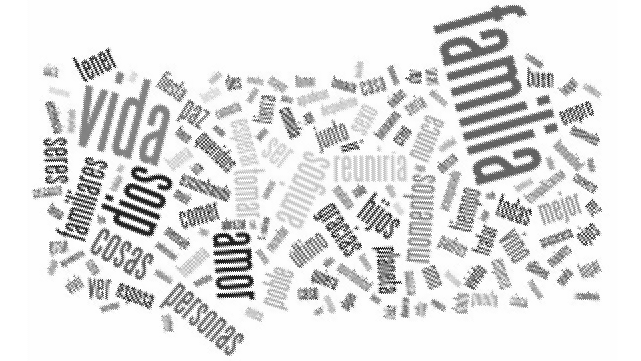
\includegraphics[scale=0.25]{imagenes/palabrask1.png}

}
\subfloat[k=3]{

	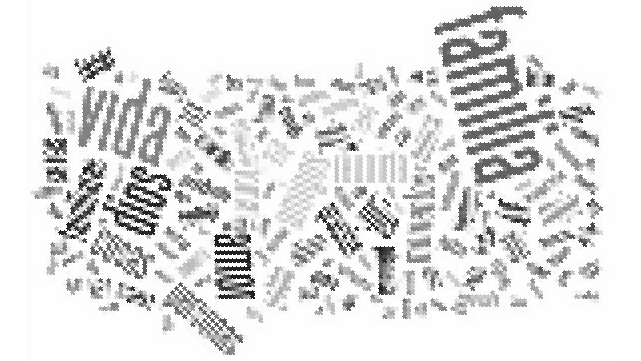
\includegraphics[scale=0.25]{imagenes/palabrask3.png}

}
\subfloat[k=4]{

	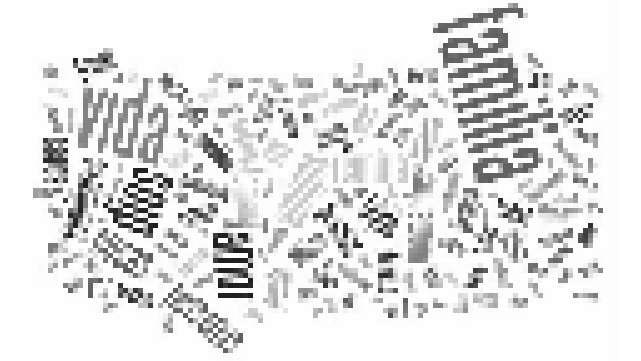
\includegraphics[scale=0.25]{imagenes/palabrask4.png}

}

\end{center}
\caption{Perdida de calidad en la imagen en el método del vecino mas cercano version Original,  al aumentar k }
\label{calidadPalabras}
\end{figure}


En la figura~\ref{calidadPalabras} podemos apreciar como disminuye a calidad del método al ir aumentando k. Para k=1 las palabras son legibles, para k=3 solo las palabras grandes resultan legibles. Para k=4 se pierde mas calidad aun, y por ejemplo la palabra ''amigos", que resulta legible para k=3, deja de serlo.


Para la imagen de globo, se obtuvieron los siguientes resultados:


\begin{table}[H]
\centering
\begin{tabular}{|r|r|r|r|r|}
\hline
\multicolumn{1}{|c|}{k} & \multicolumn{1}{c|}{Original} & \multicolumn{1}{c|}{Dinámico} & \multicolumn{1}{c|}{Promedio} \\ \hline
1 & 35.64 & 35.64& 37.62 \\ \hline
3 & 31.92 &  29.61 & 28.55 \\ \hline
7 & 28.32 &  25.87 & 22.22 \\ \hline
15 &25.42&  22.90 & 15.74 \\ \hline
\end{tabular}
\caption{Resultados de PSNR de la imagen globo ejecutadas en las variantes del m\'etodo de vecino mas cercano.}
\label{}
\end{table}

\begin{table}[H]
\centering
\begin{tabular}{|r|r|r|r|r|}
\hline
\multicolumn{1}{|c|}{k} & \multicolumn{1}{c|}{Original} & \multicolumn{1}{c|}{Dinámico} & \multicolumn{1}{c|}{Promedio} \\ \hline
1 & 0.433569 & 0.419082& 0.475161 \\ \hline
3 & 0.202544 &  0.189253 & 0.251413 \\ \hline
7 &  0.15614 &  0.126274 & 0.192875 \\ \hline
15 &0.144155&  0.110308 & 0.180333 \\ \hline
\end{tabular}
\caption{Resultados de tiempo de la imagen globo ejecutadas en las variantes del m\'etodo de vecino mas cercano.}
\label{}
\end{table}



Cualitativamente hasta para k 3 la es indistinguible al ojo la perdida de calidad de las imágenes, y a partir de k 7, ya comienza a ser mas apreciable.

Nuevamente la métrica indica que el método mas eficiente es el Original, seguido del Dinámico y del Promedio. Para k=1 se obtiene que el método de promedio es mas eficiente. Para este ultimo puede observarse el desenfoque del mismo, que para k chico es aceptable, pero para k grande el efecto es tal que la imagen pierde su forma.

En base a los resultados obtenidos, podemos decir que el método de promedio solo es útil para k chico. En la figura~\ref{globoProm} podemos ver el efecto que causa el promedio sobre la imagen para k=15.

\begin{figure}[H]
\centering
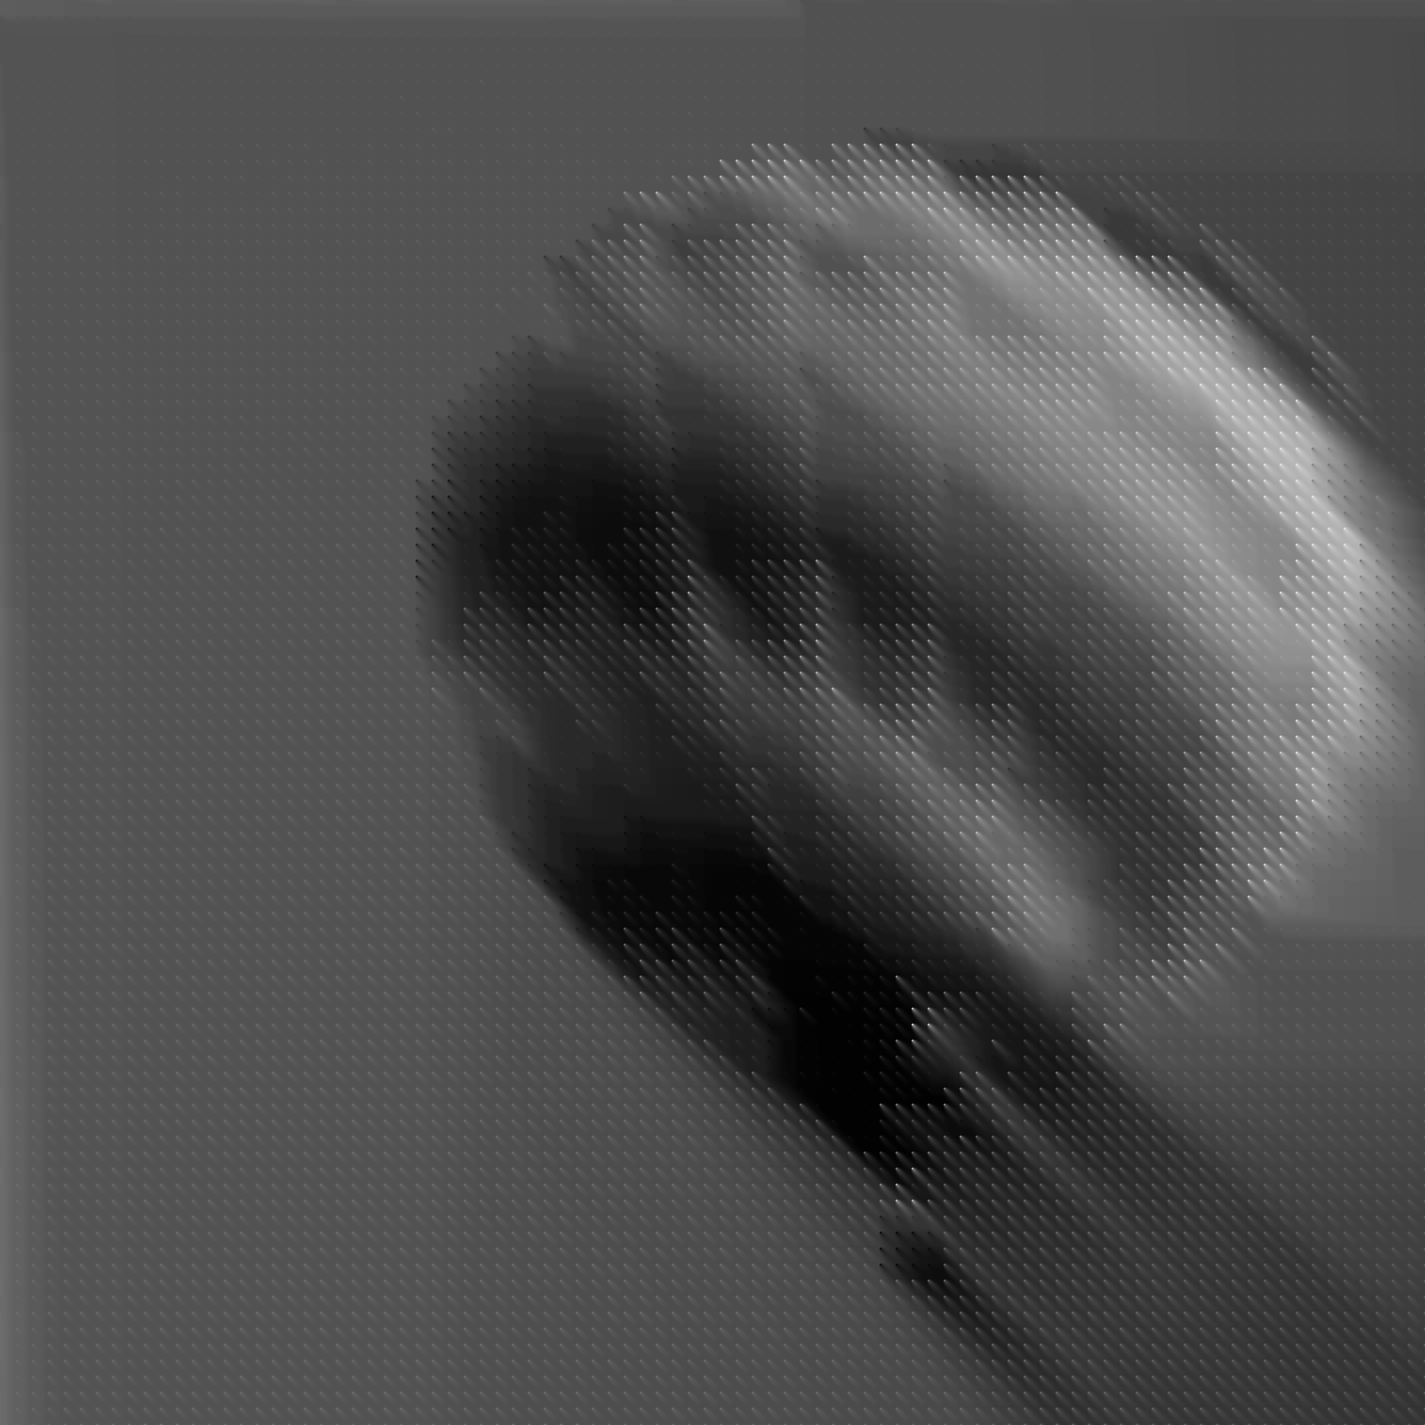
\includegraphics[scale=0.15]{imagenes/globok15.png}
\caption{Imagen obtenida para por el método de promedios para k=15}
\label{globoProm}
\end{figure}


Para la imagen de leopardo se obtuvieron los siguientes resultados para PSNR:


\begin{table}[H]
\centering
\begin{tabular}{|r|r|r|r|r|}
\hline
\multicolumn{1}{|c|}{k} & \multicolumn{1}{c|}{Original} & \multicolumn{1}{c|}{Dinámico} & \multicolumn{1}{c|}{Promedio} \\ \hline
1 & 29.49 & 29.48& 31.72 \\ \hline
2 & 28.44 &  25.92 & 26.65 \\ \hline
3 & 26.20 &  24.22 & 24.18 \\ \hline
4 &25.35&  23.14 &  22.55 \\ \hline
9 & 22.47 & 20.46& 18.06 \\ \hline
11 & 21.82 &   19.87 & 16.75 \\ \hline
14 & 21.04 &  19.08 &  14.82 \\ \hline
59 &16.92&  15.62 & 10.84 \\ \hline
\end{tabular}
\caption{Resultados de PSNR de la imagen leopardo ejecutadas en las variantes del m\'etodo de vecino mas cercano.}
\label{}
\end{table}


\begin{table}[H]
\centering
\begin{tabular}{|r|r|r|r|r|}
\hline
\multicolumn{1}{|c|}{k} & \multicolumn{1}{c|}{Original} & \multicolumn{1}{c|}{Dinámico} & \multicolumn{1}{c|}{Promedio} \\ \hline
1 & 1.0866 & 1.0504& 1.22644 \\ \hline
2 & 0.657721 &  0.61781 & 0.78355 \\ \hline
3 & 0.524817 &  0.454536& 0.638131 \\ \hline
4 &0.484191&  0.379946 &  0.559047 \\ \hline
9 & 0.37489& 0.295424& 0.46353 \\ \hline
11 & 0.368663 &   0.280538 & 0.45557 \\ \hline
14 & 0.360687 &   0.276276 &  0.441304 \\ \hline
59 &0.3529086&  0.260347 & 0.432781\\ \hline
\end{tabular}
\caption{Resultados de tiempo de la imagen leopardo ejecutadas en las variantes del m\'etodo de vecino mas cercano.}
\label{}
\end{table}

Nuevamente obtenemos el mismo orden para la calidad indicada por la métrica, que tiene una excepción para k=1 y 2 , donde el promedio obtiene mayor calidad.  Se puede ver también la disminución de la calidad al aumentar k. Este efecto se puede apreciar cualitativamente. Las manchas del leopardo son visibles hasta para k=14, sin embargo es notoria la diferencia entre este ultimo valor de k y los primeros cuatro. Estos ultimos, tienen una calidad que puede considerarse muy buena.

Hasta para k=1 puede observarse el desenfoque del promedio. No obstante para k=14 el efecto distorciona a la imagen demasiado.

Se hizo una  prueba para un k grande de 59, y se obtuvo como resultado que ni siquieraera era observable el leopardo, para ninguna de las versiones.


Para la imagen de venus se obtuvieron los siguientes resultados para PSNR:


\begin{table}[H]
\centering
\begin{tabular}{|r|r|r|r|r|}
\hline
\multicolumn{1}{|c|}{k} & \multicolumn{1}{c|}{Original} & \multicolumn{1}{c|}{Dinámico} & \multicolumn{1}{c|}{Promedio} \\ \hline
1 & 33.39 & 33.39& 35.42 \\ \hline
3 & 29.98 &  28.15 & 28.42 \\ \hline
7 & 27.16 &  25.39 &  23.50 \\ \hline
15 &24.98&  23.33 &  16.26 \\ \hline
31 & 23.18 & 21.40&  8.93 \\ \hline
63 & 21.42 &   19.53 & 8.58 \\ \hline
127 & 19.66 &  17.71 &  8.51 \\ \hline
255 &17.27&  15.78 & 8.50 \\ \hline
\end{tabular}
\caption{Resultados de PSNR de la imagen venus ejecutadas en las variantes del m\'etodo de vecino mas cercano.}
\label{}
\end{table}

\begin{table}[H]
\centering
\begin{tabular}{|r|r|r|r|r|}
\hline
\multicolumn{1}{|c|}{k} & \multicolumn{1}{c|}{Original} & \multicolumn{1}{c|}{Dinámico} & \multicolumn{1}{c|}{Promedio} \\ \hline
1 & 3.45692 & 3.34598& 3.8553 \\ \hline
3 & 1.68882 &  1.48089 & 2.03063 \\ \hline
7 & 1.26326 & 1.02672 &  1.55511 \\ \hline
15 &1.17502&  0.885899&  1.4469 \\ \hline
31 & 1.1376 & 0.873169&  1.42114 \\ \hline
63 & 1.13693 &   0.838262& 1.40754 \\ \hline
127 & 1.12636 &  0.828674 &  1.39681 \\ \hline
255 &1.13641&  0.831078 & 1.43211 \\ \hline
\end{tabular}
\caption{Resultados de tiempo de la imagen venus ejecutadas en las variantes del m\'etodo de vecino mas cercano.}
\label{}
\end{table}



Nuevamente obtenemos que según la métrica el método de mayor calidad es el Original, seguido del Dinamico, y el Promedio. También para los primeros k probados el método de promedio tiene mayor calidad. A partir de k=31 la imagen obtenida por este ultimo método es demasiado oscura y casi ni se ve, cuando para los otros dos métodos la imagen tiene una calidad aceptable. Este ultimo hecho se lo podriamos atribuir a que la imagen tiene bordes negros alrededor del planeta venus, que se promedian con la imagen. En los demas promedios puede verse el efecto de desenfoque del promedio.

Al ser una imagen de alta calidad, para los primeros k considerados y los métodos Original y Dinámico , el resultado obtenido es indistinguible a los ojos de la imagen original.

\subsection{Bilineal}
La experimentaci\'on empezar\'a aplicando zoom con k = 2 a todas las im\'agenes, y luego empezaremos a variar el k para las \'ultimas 3 im\'agenes, ya que al ser grande, hay mayor cantidad de k v\'alidos.
Se dispuso de una serie de experimentaciones sobre el siguiente conjunto de 10 imagenes:\\
\begin{itemize}
	\item Las im\'agenes \texttt{imagen1.tiff} de 511x511, \texttt{imagen2.tiff} de 1024x1024 y \texttt{imagen3.tiff} de 511x511 fueron elegidas por ser medianas y no poseer tanto cambio de colores muy marcados.
	\item Las im\'agenes \texttt{imagen4.tiff} de 1024x1024 y \texttt{imagen7.tiff} de 511x511 fueron elegidas por ser medianas y por tener personas en las mismas.
	\item Las im\'agenes \texttt{imagen5.tiff} de 1024x1024 y \texttt{imagen6.tiff} de 511x511 fueron elegidas por ser medianas y por tener muchas variaciones de colores.
	\item La imagen \texttt{imagen8.tiff} de 3289x3289 fue elegida por ser grande y por tener personas en la misma.
	\item La imagen \texttt{imagen9.tiff} de 3997x3997 fue elegida por ser grande y por tener muchas variaciones de colores.
	\item La imagen \texttt{imagen9.tiff} de 4202x4303 fue elegida por ser grande y no poseer tanto cambio de colores muy marcados.
\end{itemize}
Las im\'agenes utilizadas para este experimento se pueden encontrar en...\\

Con k=2, obtuvimos los siguiente resultados de PSNR:\\
\begin{table}[H]
\centering
\begin{tabular}{|r|r|r|r|r|}
\hline
\multicolumn{1}{|c|}{Imagenes} & \multicolumn{1}{c|}{Original} & \multicolumn{1}{c|}{Ignorando} & \multicolumn{1}{c|}{Diagonal} & \multicolumn{1}{c|}{Bloques} \\ \hline
1 & 32.6180 & 30.0720 & 31.7492 & 32.6217 \\ \hline
2 & 32.0807 &  31.3422 & 31.8774 & 32.0938 \\ \hline
3 & 34.4520 &  32.9934 & 34.4501 &  34.4509 \\ \hline
4 & 27.7731 & 23.6071 & 26.8081 & 27.7777 \\ \hline
5 & 21.9590 &  19.7860 & 21.7686 & 21.9598 \\ \hline
6 & 20.9380 & 19.7715 & 20.7258 &  20.9392 \\ \hline
7 & 29.9870 & 26.6496 & 29.3290 & 29.9945 \\ \hline
8 & 37.0023 & 31.9828 & 36.2431 & 37.0397 \\ \hline
9 & 24.0090 & 21.4330 & 23.6539 & 24.0111 \\ \hline
10 & 34.9894 & 31.8309 & 34.9878 & 34.9894 \\ \hline
\end{tabular}
\caption{Tabla de PSNR de las 10 im\'agenes ejecutadas en las 4 variantes del m\'etodo de interpolaci\'on bilineal}
\label{}
\end{table}
Con k=2, obtuvimos los siguiente resultados de tiempo(en segundos):\\
\begin{table}[H]
\centering
\begin{tabular}{|r|r|r|r|r|}
\hline
\multicolumn{1}{|c|}{Imagenes} & \multicolumn{1}{c|}{Original} & \multicolumn{1}{c|}{Ignorando} & \multicolumn{1}{c|}{Diagonal} & \multicolumn{1}{c|}{Bloques} \\ \hline
1 & 5.60 & 4.96 & 4.92 & 5.08 \\ \hline
2 & 5.90 &  5.93 & 5.91 & 5.96 \\ \hline
3 & 4.96 &  4.92 & 4.93 &  4.94 \\ \hline
4 & 6.44 & 6.00 & 5.95 & 6.00 \\ \hline
5 & 5.91 &  5.92 & 5.90 & 5.92 \\ \hline
6 & 4.93 & 4.98 & 4.93 &  4.95 \\ \hline
7 & 4.92 & 4.93 & 4.91 & 4.94 \\ \hline
8 & 18.21 & 18.52 & 17.75 & 18.90 \\ \hline
9 & 24.35 & 24.44 & 23.82 & 24.55 \\ \hline
10 & 27.07 & 27.11 & 26.52 & 27.43 \\ \hline
\end{tabular}
\caption{Tabla de tiempos de las 10 im\'agenes ejecutadas en las 4 variantes del m\'etodo de interpolaci\'on bilineal}
\label{}
\end{table}
Variando el k, con las im\'agenes \texttt{imagen8.tiff}, \texttt{imagen9.tiff} y \texttt{imagen10.tiff} se obtuvieron los siguientes resultados:\\
Con la imagen \texttt{imagen8.tiff}:\\
\begin{table}[H]
\centering
\begin{tabular}{|r|r|r|r|r|}
\hline
\multicolumn{1}{|c|}{k} & \multicolumn{1}{c|}{Original} & \multicolumn{1}{c|}{Ignorando} & \multicolumn{1}{c|}{Diagonal} & \multicolumn{1}{c|}{Bloques} \\ \hline
3 & 34.1484 & 29.3108 & 33.3469 & 34.1729 \\ \hline
5 & 30.6667 &  26.8999 & 30.1220 & 30.6836 \\ \hline
7 & 28.3968 &  25.3233 & 27.9253 &  28.4112 \\ \hline
\end{tabular}
\caption{Tabla de PSNR de la imagen8 ejecutadas en las 4 variantes del m\'etodo de interpolaci\'on bilineal, variando el k en 3, 5 y 7.}
\label{}
\end{table}
\begin{table}[H]
\centering
\begin{tabular}{|r|r|r|r|r|}
\hline
\multicolumn{1}{|c|}{k} & \multicolumn{1}{c|}{Original} & \multicolumn{1}{c|}{Ignorando} & \multicolumn{1}{c|}{Diagonal} & \multicolumn{1}{c|}{Bloques} \\ \hline
3 & 17.73 & 17.27 & 16.60 & 17.47 \\ \hline
5 & 16.37 &  16.25 & 15.67 & 16.78 \\ \hline
7 & 15.92 &  16.06 & 15.70 &  16.65 \\ \hline
\end{tabular}
\caption{Tabla de tiempos de la imagen8 ejecutadas en las 4 variantes del m\'etodo de interpolaci\'on bilineal, variando el k en 3, 5 y 7.}
\label{}
\end{table}
Con la imagen \texttt{imagen9.tiff}:\\
\begin{table}[H]
\centering
\begin{tabular}{|r|r|r|r|r|}
\hline
\multicolumn{1}{|c|}{k} & \multicolumn{1}{c|}{Original} & \multicolumn{1}{c|}{Ignorando} & \multicolumn{1}{c|}{Diagonal} & \multicolumn{1}{c|}{Bloques} \\ \hline
3 & 22.4157 & 19.8676 & 22.1082 & 22.4174 \\ \hline
5 & 20.4671 & 18.0751 & 20.1985 &  20.4688 \\ \hline
8 &  18.7939 &  16.5599 & 18.5421 & 18.7957 \\ \hline
\end{tabular}
\caption{Tabla de PSNR de la imagen9 ejecutadas en las 4 variantes del m\'etodo de interpolaci\'on bilineal, variando el k en 3, 5 y 8.}
\label{}
\end{table}
\begin{table}[H]
\centering
\begin{tabular}{|r|r|r|r|r|}
\hline
\multicolumn{1}{|c|}{k} & \multicolumn{1}{c|}{Original} & \multicolumn{1}{c|}{Ignorando} & \multicolumn{1}{c|}{Diagonal} & \multicolumn{1}{c|}{Bloques} \\ \hline
3 &  22.93 &  23.26 &  22.55 & 23.81 \\ \hline
5 & 22.04 & 21.95 & 21.58 &  22.14 \\ \hline
8 &  21.83 &  21.15 & 19.93 & 21.55 \\ \hline
\end{tabular}
\caption{Tabla de tiempos de la imagen9 ejecutadas en las 4 variantes del m\'etodo de interpolaci\'on bilineal, variando el k en 3, 5 y 8.}
\label{}
\end{table}

Con la imagen \texttt{imagen10.tiff}:\\
\begin{table}[H]
\centering
\begin{tabular}{|r|r|r|r|r|}
\hline
\multicolumn{1}{|c|}{k} & \multicolumn{1}{c|}{Original} & \multicolumn{1}{c|}{Ignorando} & \multicolumn{1}{c|}{Diagonal} & \multicolumn{1}{c|}{Bloques} \\ \hline
1 & 38.2838 & 34.9337 &  38.2821 &  38.2838 \\ \hline
5 & 30.9075 & 27.6721 & 30.9051 &  30.9075\\ \hline
8 &  27.4966 &   25.3160 & 27.4906 &  27.4967 \\ \hline
\end{tabular}
\caption{Tabla de PSNR de la imagen10 ejecutadas en las 4 variantes del m\'etodo de interpolaci\'on bilineal, variando el k en 1, 5 y 8.}
\label{}
\end{table}
\begin{table}[H]
\centering
\begin{tabular}{|r|r|r|r|r|}
\hline
\multicolumn{1}{|c|}{k} & \multicolumn{1}{c|}{Original} & \multicolumn{1}{c|}{Ignorando} & \multicolumn{1}{c|}{Diagonal} & \multicolumn{1}{c|}{Bloques} \\ \hline
1 & 33.77 &  33.33 & 32.35 & 33.02 \\ \hline
5 & 23.48 &  23.47 & 22.77 & 24.43 \\ \hline
8 & 23.42 &  23.55 & 21.65 &  23.75 \\ \hline
\end{tabular}
\caption{Tabla de tiempos de la imagen10 ejecutadas en las 4 variantes del m\'etodo de interpolaci\'on bilineal, variando el k en 1, 5 y 8.}
\label{}
\end{table}

Es importante destacar que el tiempo de computo no se vio afectado por las variantes del m\'etodo, sino solamente, como era de esperar, por el tamaño de cada imagen.\\
Luego de analizar los resultados objetivos, procederemos a analizar subjetivamente las imagenes.\\
Con k=2, en las variantes del m\'etodo original, por diagonales y por bloques se pudo observar un cierto efecto de desenfoque de la imagen en donde los contornos de los objetos no estaban bien definidos. Esto se ve en todas las imagenes excepto en la imagen5, que se nota muy despixelada, seguramente debido a la cantidad de colores y letras que presenta la misma.
La siguiente comparaci\'on muestra lo recientemente enunciado.\\


    \begin{figure}[H]
    \centering
    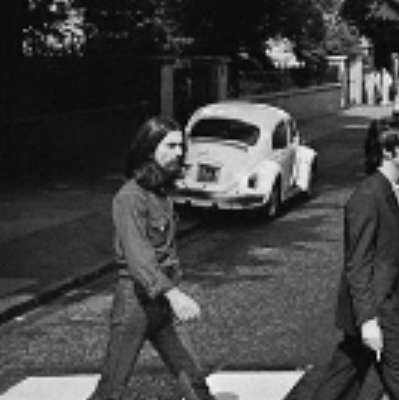
\includegraphics[scale=0.5]{imagenes/imagen4informe.png}
    \caption{Fracci\'on Imagen 4 - Bilineal por bloques}
    \end{figure}

     \begin{figure}[H]
    \centering
    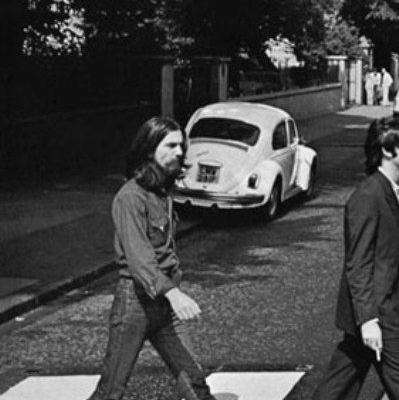
\includegraphics[scale=0.5]{imagenes/imagen4informeOriginal.png}
    \caption{Fracci\'on Imagen 4 - Orginal}
    \end{figure}

     \begin{figure}[H]
    \centering
    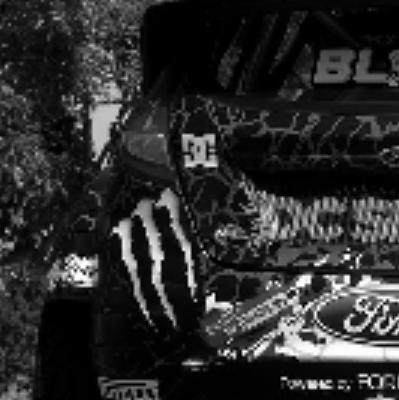
\includegraphics[scale=0.5]{imagenes/imagen5informe.png}
    \caption{Fracci\'on Imagen 5 - Bilineal por bloques}
    \end{figure}

     \begin{figure}[H]
    \centering
    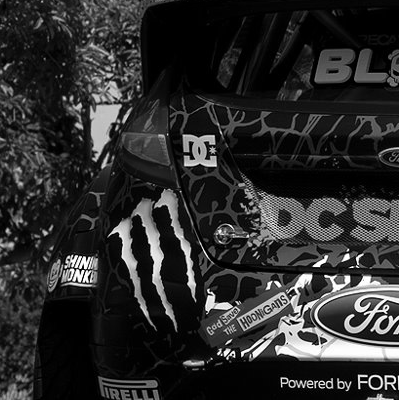
\includegraphics[scale=0.5]{imagenes/imagen5informeOriginal.png}
    \caption{Fracci\'on Imagen 5 - Orginal}
    \end{figure}

Tambien es notable que el m\'etodo con la variante de ignorar un pixel, en las imagenes que varia el color seguido, deja m\'as detalles especiales de lo que esperabamos, como una imagen despixelada, o con franjas blancas y negras, que si le aplic\'aramos zoom con el visor de imagenes tradicional, queda al descubierto una trama negra m\'as notoria. En cambio en las que no var\'ia el color seguido, deja imagenes aceptables. En la siguiente comparaci\'on se observa lo recientemente detallado.\\ Esto concuerda tambien con los valores resultantes del PSNR calculado. En donde con la variante de ignorar un pixel, la imagen 4 obtuvo casi 4 puntos menos de PSNR comparado con las otras variantes, mientras que la imagen 2 obtuvo similar valor para todas las variantes.\\
 \begin{figure}[H]
    \centering
    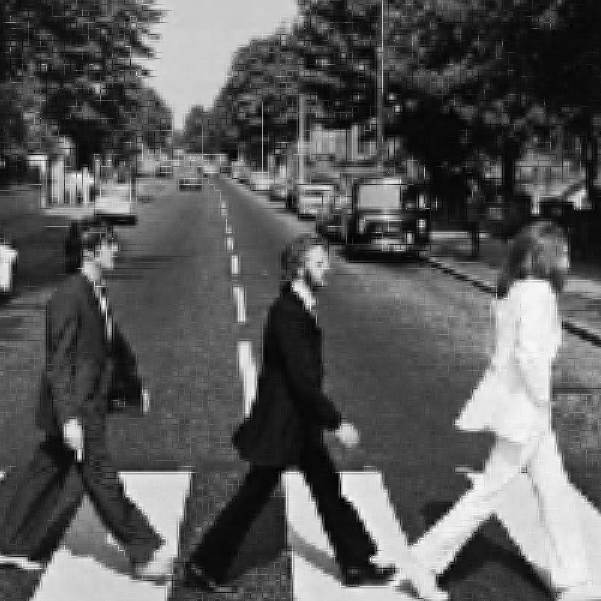
\includegraphics[scale=0.5]{imagenes/imagen4informe2.png}
    \caption{Fracci\'on Imagen 4 - Bilineal ignorando un pixel}
    \end{figure}

     \begin{figure}[H]
    \centering
    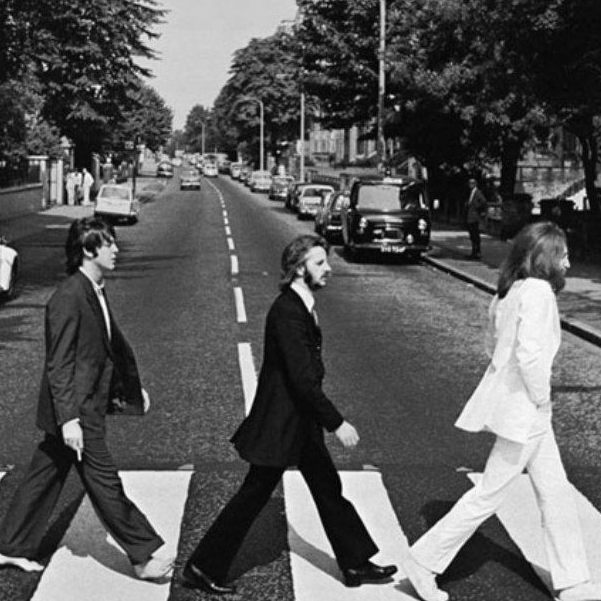
\includegraphics[scale=0.5]{imagenes/imagen4informe2Original.png}
    \caption{Fracci\'on Imagen 4 - Orginal}
    \end{figure}

     \begin{figure}[H]
    \centering
    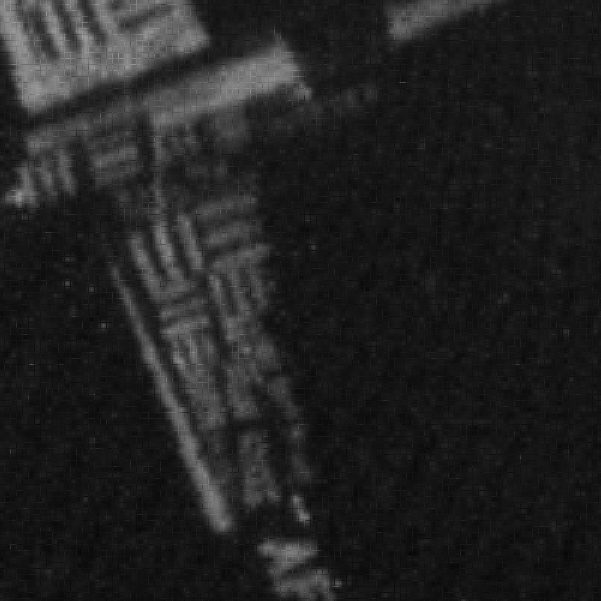
\includegraphics[scale=0.5]{imagenes/imagen2informe.png}
    \caption{Fracci\'on Imagen 2 - Bilineal por bloques}
    \end{figure}

     \begin{figure}[H]
    \centering
    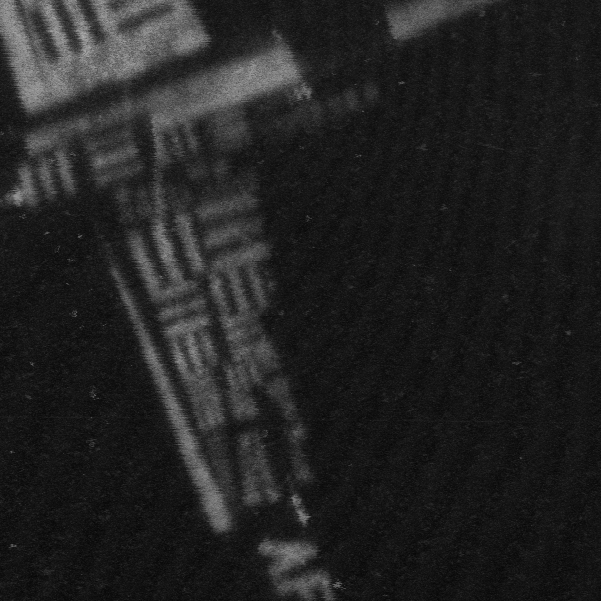
\includegraphics[scale=0.5]{imagenes/imagen2informeOriginal.png}
    \caption{Fracci\'on Imagen 2 - Orginal}
    \end{figure}
Comparando las variantes original, por diagonal y por bloques sobre cada una de las otras im\'agenes, no se noto diferencias visibles al sentido humano comparando cada una de ellas, es decir comparando la misma foto pero con diferentes variantes.
De pudo apreciar, que para las imagenes grandes a medida que aumentamos el k ayud\'andonos con la opci\'on del zoom del visor de imagenes del visor de im\'agenes tradicional, las mismas contenian un desenfoque cada vez m\'as notorio. Esto se envidenci\'o notablemente en la \texttt{imagen9.tiff}, ademas dio un valor bajo de PSNR en comparaci\'on a las otras 2 im\'agenes grandes, posiblemente a causa de la gran cantidad de variaciones de colores muy seguidas.\\


 Con las im\'agenes donde no hab\'ia cambios tan seguidos de colores, se pudo verificar que la variante de ignorar un pixel, retorno un valor similar de PSNR, con diferencias de 1 0 2 puntos en relaci\'on a las otras variantes. Nunca se obtuvo mejor valor de PSNR.
 En cuanto con las im\'agenes que si tenian cambios seguidos de color, el valor de PSNR dio muy por debajo de lo que dieron las otras variantes, llegando a diferencias de entre 4 y 6 puntos. Ademas se encontraron artifacts muy notorios en las im\'agenes como los expuestos en la secci\'on de resultados.\\
 Tambien mostramos que la variante original y la de por bloques, casi devolvieron similares valores de PSNR, con minimas diferencias, siempre obteniendo mayor valor la variante por bloques. Suponiamos que iban a dar similares pero que la variante original iba a dar siempre mejor que por bloques debido a que en la implementaci\'on se realizan menos casteos de variables y eso podria haber arrastrado errores de precisi\'on.\\
 En cuanto a los valores de PSNR de la variante de diagonales, siempre obtuvimos valores con diferencias de a lo sumo 1 punto, lo que marcar\'ia que las im\'agenes elegidas posiblemente no tengan una continuidad diagonal de color en todos los sectores.\\
 Para destacar es que los resultados arrojaron que a medida que el k aumenta, si la imagen posee bastantes cambios abruptos de colores, se obtendr\'an imagenes con menos calidad objetiva y subjetiva.\\
 Tambien observamos que el tiempo de computo no se vio alterado al cambiar de variante, por lo que podemos asegurar que solo el tamaño de cada imagen influye en el mismo.\\
 Para finalizar con el estudio de este metodo, concluimos que la mejor variante en cuanto calidad objetiva y calidad subjetiva es la variante por bloques.

\subsection{Splines}
\label{Splines}

Como mencionamos anteriormente en el desarrollo, implementamos dos variantes distintas de este método y por lo tanto experimentamos con ambas variantes. Las imágenes seleccionadas se encuentran en la carpeta Experimentación/Splines y a continuación explicaremos qué particularidad tiene cada imagen junto con los k que vamos a trabajar.
\newline
\newline Tanque: esta imagen fue elegida para ver como afecta en los resultados el hecho de tener todo un terreno relativamente uniforme junto con un objeto más o menos mediano (en este caso el tanque), de tonalidad similar. Al igual que Cuadrícula y Grises, las dimensiones de esta imagen son 511x511 y trabajaremos con $k = 1, 2$ y $4$.
\newline \newline Cuadrícula: nos pareció interesante incluir esta imagen por el hecho de contener, en su mayor parte, cuadrados y así poder ver el comportamiento del algoritmo de splines por bloques de tamaño fijo. Además como está compuesta básicamente por líneas, podemos ver que tan tolerante es al $k$, es decir, cuanta información se pierde.
\newline \newline Grises: al igual que Cuadrícula, esta imagen se puede dividir pero en rectángulos y es interesante ver si el algoritmo por bloques fijos puede funcionar relativamente bien, ya que los bloques que usa deben ser necesariamente cuadrados. Además, dado que existe un cambio de tonalidad por cada rectángulo adyacente, esto puede significar una experimentación interesante en la variante de bloques de tamaño variable porque sirve para evaluar que tan bien puede identificar ese cambio de tonalidad.
\newline \newline Lago: 
\newline \newline Auto y Rosa: elegimos estas imágenes por el nivel de detalle que contienen. El auto sobre todo, tiene una cantidad importante de iluminación y reflejos, cosa que ninguna otra imagen hasta ahora tenía. Las dimensiones de Auto (4096x4096) nos permiten trabajar con varios valores de $k$ que serán 2, 4, 6, 8 y 12 mientras que con Rosa (2047x2047) vamos a usar $k = 1, 2, 5$.
\newline \newline Piano: esta imagen fue elegida para ver como se comportan los algoritmos tanto con el reflejo de las teclas (que está bien delimitado) como con los bordes de las mismas. Sus dimensiones son 1549x1549 y trabajaremos con $k = 1, 2, 3$.

Si bien presentamos algunos recortes de las imágenes utilizadas en esta sección que ilustran las diferencias más relevantes entre la imagen original y las imágenes procesadas por el algoritmo, también mencionamos otras diferencias importantes que, por cuestiones de espacio y claridad, preferimos decir donde se encuentran y que se vean directo de las imágenes adjuntas al trabajo.
Ahora que ya explicamos los aspectos que van a compartir las experiencias de ambas variantes, pasamos a hablar específicamente de la variante del método que utiliza bloques de tamaño fijo. La idea va a ser tratar de ver las diferencias en las imágenes al tomar bloques de un tamaño u otro, eligiendo estos tamaños en base a la imagen con la cual vamos a estar trabajando. El enfoque que adoptaremos en general va a ser el siguiente: dada una imagen y un $k$, aplicar el método una vez con un bloque del tamaño de la imagen y otra vez con bloques de cierto tamaño, que será decidido según ciertos aspectos de la imagen. Por ejemplo, si la imagen es relativamente parecida en todas partes (porque se trata de un terreno por ejemplo) salvo por un area delimitada, el tamaño del bloque va a ser el tamaño de este area. De esta manera, estamos separando de alguna manera a la parte que difiere en la imagen de las partes que son parecidas. Decimos en general porque en algunos casos no se va a cumplir que la imagen posea esta uniformidad y ahí va a ser cuando cambiemos un poco este enfoque. En casos donde la imagen posee muchos detalles y es muy cambiante, vamos a tomar bloques de tamaño chico bajo la hipótesis de que como es probable que de un bloque a otro la imagen cambie significativamente, al tomar bloques reducidos vamos a estar descartando información sobre otra parte de la imagen que no aporta al area que queremos procesar, porque justamente en esa otra parte la imagen pudo haber cambiado mucho.

Comencemos analizando los resultados obtenidos para las imágenes de 511x511. Para la imagen Tanque.tiff, utilizamos bloques de un tamaño que aproxima a la mitad del tanque (esto es debido a que el tanque es rectangular y los bloques deben ser cuadrados por como está diseñado el algoritmo). Haciendo un análisis cualitativo de nuestras imágenes, comenzando por las que se procesaron con $k = 1$, podemos observar que entre la que trabaja con un bloque del tamaño entero de la imagen (256x256) y la que trabaja con bloques de 50x50 practicamente no hay diferencias que se puedan percibir fácilmente de manera visual. Si tratamos de ver muy detenidamente las diferencias entre ambas, podemos encontrar que, en la parte más oscura del tanque (más o menos por la mitad izquierda) la imagen procesada con bloques de 256 remarca un poco más el blanco del borde. Sin embargo, como ya dijimos, es practicamente imperceptible. Lo que sí se puede percibir notoriamente es la diferencia entre cualquiera de estas imágenes y la imagen original. Lo que más llama la atención son los detalles del tanque que se pierden totalmente, por ejemplo las lineas negras que tiene en la parte de arriba que se borronean. En la parte del cañón se produce un despixelado bastante fuerte, probablemente mayor al que se produce en las otras partes del tanque como por ejemplo en la de abajo donde están las ruedas. Una de las razones posibles que podrían explicar esto es que, justamente, los píxeles del cañón están aislados del resto del tanque y sus vecinos más cercanos corresponden a los píxeles del terreno, entonces por más que tomemos un bloque grande de 256x256 o bloques del tamaño de la mitad del tanque, seguramente en el/los bloque/s correspondiente/s al cañón del tanque van a estar tanto los píxeles del cañón como los del terreno y, seguramente van a predominar estos últimos. Obsevermos que en las lineas negras que mencionamos al principio sucede algo similar, se pierde mucha de esa información debido a que las líneas son muy finas y por lo tanto, en el bloque que tomemos que contengan estas líneas, van a predominar los píxeles grises. Todo esto sumado a que cuando realizamos la reducción del tamaño de la imagen ya se pierde una cantidad de información significativa y las partes donde están los detalles se ven más afectadas.
\par Para $k = 2$ y $k = 4$ lo que sucede es que las diferencias que notamos para $k = 1$ tanto entre las imágenes con zoom como entre alguna de ellas y la original aumentan bastante. En el caso particular de $k = 2$ ahora quizás es más fácil identificar diferencias entre la imagen aumentada con un bloque de 171 y la procesada con bloques de 30 sobre todo en la parte de las ruedas del tanque. Sin embargo, lo más relevante es que ahora la parte del cañón ya se comienza a confundir con el terreno. Y si pasamos a $k = 4$, para ambas imágenes, el cañón ya se perdió por completo.
\begin{figure}[H]
\centering
\subfloat[Original]{
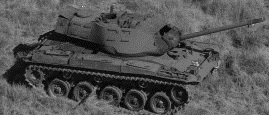
\includegraphics[scale=0.5]{imagenes/ImgsSplinesBloquesFijos/tanqueorig.jpg}
}
\subfloat[k = 1, bloques de 50x50]{
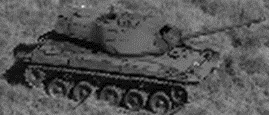
\includegraphics[scale=0.5]{imagenes/ImgsSplinesBloquesFijos/tanque50.jpg}
}
\subfloat[k = 2, bloques de 30x30]{
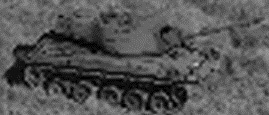
\includegraphics[scale=0.5]{imagenes/ImgsSplinesBloquesFijos/tanque30.jpg}
}
\subfloat[k = 4, bloques de 20x20]{
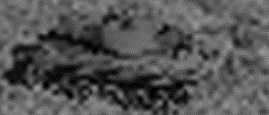
\includegraphics[scale=0.5]{imagenes/ImgsSplinesBloquesFijos/tanque20.jpg}
}
\caption{Comparación entre la imagen original y la procesada con distintos $k$ y tamaños de bloque chicos}
\end{figure}

\begin{figure}[H]
\centering
\subfloat[Bloques de 50x50]{
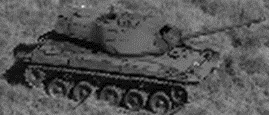
\includegraphics[scale=0.5]{imagenes/ImgsSplinesBloquesFijos/tanque50.jpg}
}
\subfloat[Un solo bloque de 256x256]{
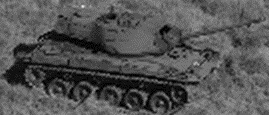
\includegraphics[scale=0.5]{imagenes/ImgsSplinesBloquesFijos/tanque256.jpg}
}
\caption{Comparación en base al tamaño de los bloques para k = 1}
\end{figure}

\begin{figure}[H]
\centering
\subfloat[Bloques de 30x30]{
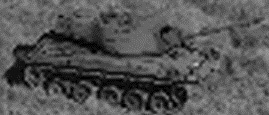
\includegraphics[scale=0.5]{imagenes/ImgsSplinesBloquesFijos/tanque30.jpg}
}
\subfloat[Un solo bloque de 171x171]{
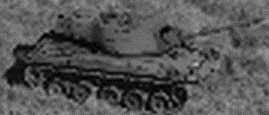
\includegraphics[scale=0.5]{imagenes/ImgsSplinesBloquesFijos/tanque171.jpg}
}
\caption{Comparación en base al tamaño de los bloques para k = 2}
\end{figure}

\begin{figure}[H]
\centering
\subfloat[Bloques de 20x20]{
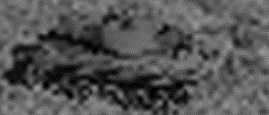
\includegraphics[scale=0.5]{imagenes/ImgsSplinesBloquesFijos/tanque20.jpg}
}
\subfloat[Un solo bloque de 103x103]{
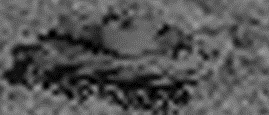
\includegraphics[scale=0.5]{imagenes/ImgsSplinesBloquesFijos/tanque103.jpg}
}
\caption{Comparación en base al tamaño de los bloques para k = 4}
\end{figure}

\par En resumen, pareciera que las diferencias entre las imágenes procesadas con bloques relativamente chicos en relación al tamaño de las imágenes y las que se procesan con un bloque del tamaño de la imagen, van aumentando de a poco a medida que aumentamos el $k$. Si bien procesarlas de una u otra manera no evita (al menos en este caso) los problemas más relevantes (como el despixelado o que se confunda totalmente una parte de la imagen con el resto de los píxeles la rodean), existen algunas pequeñas diferencias como por ejemplo en las ruedas del tanque. Dado que estas diferencias no son visualmente muy relevantes, no podemos estar seguros de si contribuyen a una reconstrucción mejor o peor de la imagen ya que son diferencias muy pequeñas. Para resolver esto vamos a cuantificar un poco las cosas, a continuación mostramos el PSNR de cada imagen junto con el tiempo de cómputo que llevó procesarla:
\newline

\centerline{
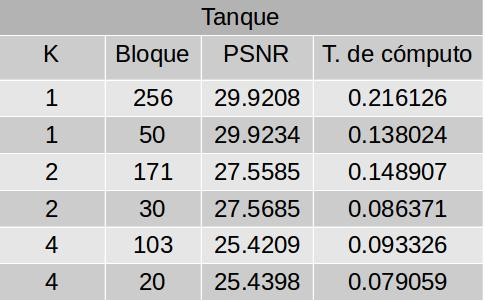
\includegraphics[scale=0.5]{imagenes/tanqueTabla.jpg}
}

Podemos ver como el análisis cualitativo que habíamos hecho sobre las imágenes, concuerda bastante con los números presentados en la tabla. Para empezar, vemos como efectivamente a medida que aumentamos el $k$ el PSNR decrece y eso significa que el error entre la imagen esperada y la resultante es mayor. También es cierto que las diferencias entre las imágenes procesadas con un bloque y las que procesamos con varios bloques aumentan a medida que aumenta el $k$ ya que para $k = 1$ la diferencia es de 0.0026, para $k = 2$ de 0.01 y para $k = 4$ de 0.0189. Lo interesante de esto es que dado que estas diferencias son muy chicas, no eramos capaces de decidir si estaban ayudando a reconstruir mejor o peor la imagen porque visualmente era muy dificil. Ahora podemos ver que, en los tres casos el PSNR es mayor cuando trabajamos la imagen con bloques del tamaño de la mitad del tanque.
\par En cuanto al tiempo de cómputo, se observa que si bien todos los tiempos medidos son bastante chicos, al trabajar con las imágenes reducidas de mayor tamaño ($k$ chico), el tiempo es mayor. Si bien trabajar con cualquier valor de $k$ va a resultar en una imagen expandida del mismo tamaño, lo que sucede al trabajar con $k$ pequeños es que los splines que se van a ir generando van a tener más información, con lo cual van a demandar un costo computacional más grande. Esto se puede ver también por la diferencia de tiempos que existe, para un mismo $k$, cuando se trabaja con bloques de tamaño chico y cuando se trabaja con un bloque grande. La tabla muestra que, en el primer caso, los tiempos son menores, lo que significa que concuerda con lo que dijimos recién, ya que al trabajar con bloques pequeños, si bien vamos a generar más splines, van a tener menos información. Por lo tanto una posible hipótesis en cuanto al tiempo de cómputo es que generar cierta cantidad de splines con muchos puntos es más costoso que generar quizás, una mayor cantidad pero con menos puntos cada uno.


Pasemos ahora a analizar la imagen Grises y veamos si sucede algo parecido a lo que pasó con la anterior. Para esta imagen, al igual que la anterior, vamos a trabajar con bloques de un tamaño cercano al tamaño de los rectángulos (además del caso de trabajar con un solo bloque que siempre lo usamos). En este caso vuelve a pasar que las diferencias entre las imágenes que trabajan con muchos bloques y las que trabajan con un solo bloque aumentan a medida que aumenta el $k$. Comenzando por $k = 1$, podemos ver que el tercer y cuarto rectángulos de la primera columna (en los otros es dificil de ver esto) difieren levemente entre la imagen 256 y 38: en el primer caso pareciera estar cubierto por líneas horizontales y en el extremo derecho también por líneas verticales, mientras que en el segundo caso pasa algo parecido pero en la parte de arriba de esos rectángulos no existen esas líneas. En principio es dificil tratar de pensar un posible motivo por el cual sucede esto ya que solo es apreciable en algunas partes de la imagen y no en todas. En cuanto a las diferencias con la imagen original, podemos observar que existe una leve variación entre el tamaño de los rectángulos: en la original los rectángulos de la columna izquierda y derecha parecieran ser un tanto más chicos que los de las imágenes resultantes y el del medio un poco más grande. Para $k = 2$ la diferencia en los tamaños de los rectángulos entre las imágenes resultantes y la imagen original es significativamente más notoria al igual que el cuadriculado que observamos antes en algunos rectángulos, que ahora se puede observar en otros como los que se encuentran más cercanos al centro de la imagen. Finalmente para $k = 4$ podemos ver que los dos defectos que nombramos antes se potenciaron bastante al igual que las diferencias entre las imágenes procesadas. A grandes rasgos se puede notar que la mayor parte de los rectángulos de la imagen 103 posee una especie de cuadriculado mientras que los de la imagen 38 solo líneas, en los extremos de ambos casos varía levemente este patrón. Vemos que al igual que nos pasó con la imagen Tanque, si bien existen diferencias entre la imagen procesada con un bloque solo y la que procesada con varios bloques, ambas comparten un defecto mayor que es el cambio en el tamaño de los rectángulos que es lo más apreciable a la vista. 
\noindent A continuación presentamos la tabla con los resultados sobre el tiempo de cómputo y el PSNR:
\newline

\centerline{
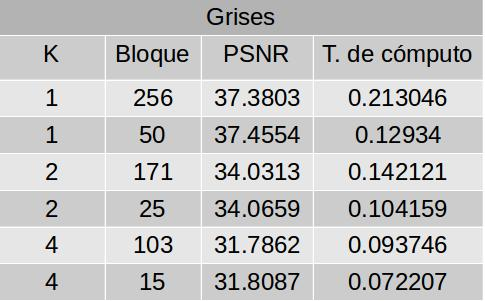
\includegraphics[scale=0.5]{imagenes/grisesTabla.jpg}
}

Si bien el procesamiento por bloques sigue siendo superior al procesamiento con un solo bloque en términos de PSNR, al igual que con la imagen Tanque, aca la diferencia entre el PSNR de una y de otra va disminuyendo a medida que aumenta el $k$, a diferencia del caso anterior. Visualmente esto tiene algún sentido ya que, tanto en un caso o en otro a medida que el $k$ aumentaba el rayado y el cuadrículado se hacían cada vez más visibles.
\par Con respecto al tiempo de cómputo, no tiene mucho sentido analizarlo mucho ya que era bastante esperable que nos de muy parecido al que tomamos con Tanque, porque estamos trabajando con una imagen de las mismas dimensiones y varios de los tamaños de los bloques son los mismos y otros son muy parecidos.

Ahora vamos a presentar el análisis correspondiente a la última imagen de 511, Cuadrícula, que representa un caso bastante patológico. Decimos esto porque al aumentar el $k$ de 1 a 2 la cantidad de información que se pierde es muy grande, lo cual es bastante lógico porque la imagen está compuesta básicamente por líneas y estas líneas contienen una cantidad de píxeles bastante reducida. Sin embargo, nos pareció una instancia interesante debido a que como el algoritmo trabaja con bloques necesariamente cuadrados y salvo por algunos pocos sectores, esta imagen es practicamente un cuadriculado, ahora ya no es necesario tomar el tamaño del bloque como la mitad de algún sector (como sucedía en las imágenes anteriores). Para $k = 1$ lo que podemos observar si miramos la imagen que fue procesada tomando bloques del tamaño del cuadrado y la que fue procesada con un solo bloque del tamaño total de la imagen, es que esta última remarca las líneas. Si miramos en detalle, además de las líneas también remarca algunas partes de los números (se puede ver fácilmente en la parte inferior de los números 2). Si bien ambas variantes reconstruyen la parte de las líneas correctamente (con sus diferencias, pero podemos decir que es visualmente aceptable), el mayor problema viene con los números. Los números del eje vertical se entienden bastante pero los del eje horizontal parecen haber perdido una cantidad de píxeles importante. Probando con otros tamaños de bloque más grandes (por ejemplo cercanos al tamaño de uno de estos números del eje horizontal o tomar bloques más chicos que uno de los cuadrados de la imagen) se puede ver que la calidad de estos números no mejora, con lo cual empezamos a pensar que no es un problema de la elección del tamaño del bloque, si no de la cantidad de información perdida a la hora de reducir la imagen.

\begin{figure}[H]
\centering
\subfloat[Original]{
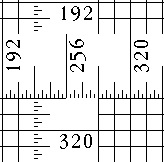
\includegraphics[scale=0.5]{imagenes/ImgsSplinesBloquesFijos/cuadriculaoriginal.jpg}
}
\subfloat[1, 9]{
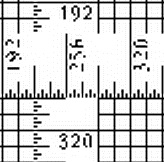
\includegraphics[scale=0.5]{imagenes/ImgsSplinesBloquesFijos/cuadriculak19.jpg}
}
\subfloat[2, 17]{
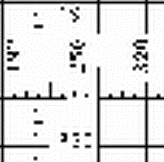
\includegraphics[scale=0.5]{imagenes/ImgsSplinesBloquesFijos/cuadriculak217.jpg}
}
\subfloat[4, 17]{
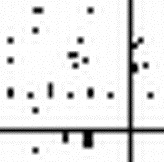
\includegraphics[scale=0.5]{imagenes/ImgsSplinesBloquesFijos/cuadriculak417.jpg}
}
\caption{Comparación entre la imagen original y la procesada con distintos $k$. Debajo de cada imagen se encuentra su respectivo $k$ y tamaño de bloque utilizado.}
\end{figure}

\begin{figure}[H]
\centering
\subfloat[Bloques de 9x9]{
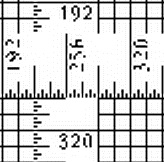
\includegraphics[scale=0.5]{imagenes/ImgsSplinesBloquesFijos/cuadriculak19.jpg}
}
\subfloat[Un solo bloque de 256x256]{
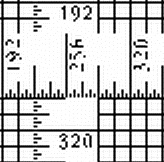
\includegraphics[scale=0.5]{imagenes/ImgsSplinesBloquesFijos/cuadriculak1256.jpg}
}
\caption{Comparación en base al tamaño de los bloques para k = 1}
\end{figure}

\par Para los casos con $k = 2$ y $k = 4$, las imágenes resultantes difieren mucho de la original porque la cantidad de información que se pierde al reducirlas es muy significativa, por el tipo de imagen que representan, esto se puede observar fácilmente al reducir la imagen original con esos valores de $k$ y ver que queda algo realmente muy distinto a lo que uno esperaría, lo cual no pasa con $k = 1$ y es por eso que el método funciona mejor. Entonces podemos concluir que la diferencia que existe entre la imagen original y las procesadas con $k = 2$ y $k = 4$ no es una consecuencia del método utilizado si no del tipo de imagen, muy sensible a reducciones.
\newline A continuación, presentamos la tabla correspondiente a esta imagen:
\newline

\centerline{
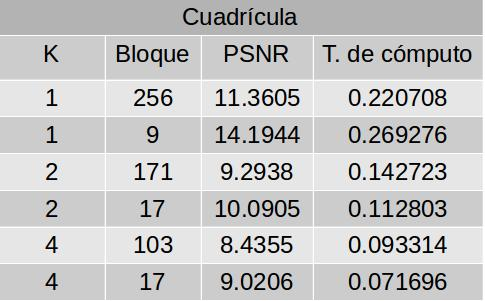
\includegraphics[scale=0.5]{imagenes/cuadriculaTabla.jpg}
}

Vemos como impacta el hecho de usar bloques del tamaño de los cuadrados para $k = 1$ (que, por lo que explicamos anteriormente sobre las reducciones, es el caso que más vale la pena analizar). Si bien visualmente la única diferencia significativa que existe entre estas imágenes es que una remarca más las líneas que la otra, éste fue el caso en el cual se pudo apreciar la mayor diferencia entre procesar por bloques y hacerlo solo con un bloque. Concluimos que esto sucedió justamente porque la imagen está dividida en cuadrados y los bloques con los que trabaja nuestro algoritmo deben ser cuadrados también.
\par En este caso, los tiempos medidos nos pueden estar diciendo algo más ya que vemos que el tiempo para $k = 1$ y un tamaño de bloque de 9 píxeles, es levemente mayor que el tiempo para un bloque de 256 y el mismo $k$. Esto contradice lo que veníamos pensando por los datos tomados de las imágenes anteriores, sin embargo, como se tratan de tiempos muy cortos y la diferencia no es demasiado grande, puede que sea un caso particular que no debe ser tenido en cuenta. Seguiremos analizando este aspecto en las próximas imágenes y probablemente nos digan algo más ya que al ser de dimensiones más grandes, los tiempos van a ser mayores.

Ahora pasaremos a analizar las imágenes más grandes, empezando por Lago. Dado que en esta imagen podemos identificar tres sectores que son el lago, el cielo y el terreno y son sectores relativamente grandes los tres (junto con la imagen en general, que también es grande), vamos a trabajar con tamaños de bloques bastante variables y no tan chicos como los de las imágenes anteriores. Además, para cambiar un poco, vamos a dejarlos fijos cuando varíe el $k$. Estos bloques van a ser de 50, 100 y 200. 
\par Visualmente lo primero que podemos decir es que esta vez sí son realmente imperceptibles las diferencias entre las imágenes procesadas con un tramaño de bloque u otro, incluso para los $k$ más grandes. Más aún, lo que sucede es que si bien las diferencias entre las imagenes resultantes y la imagen original existen y son apreciables, de alguna manera no afectan la calidad de la imagen para los primeros valores de $k$. Esto último se debe a lo que dijimos inicialmente: estamos trabajando con una imagen donde existen tres secciones bastante grandes y que además, los bordes no están bien definidos (es decir, no hay una linea bien definida que divida una sección de la otra) entonces si existe alguna diferencia en los bordes, visualmente no va a ser muy perceptible a menos que sea muy grande. porque en la imagen inicial el borde ya es irregular. A medida que se aumenta el $k$ lo que notamos es que estas diferencias en los arboles se hacen más significativas y ya en $k = 5$ y $k = 7$   el cambio es bastante grande, incluso en el terreno se nota que la calidad es mala.
\begin{figure}[H]
\centering
\subfloat[Original]{
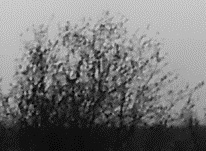
\includegraphics[scale=0.5]{imagenes/ImgsSplinesBloquesFijos/lagooriginal1.jpg}
}
\subfloat[1, 525]{
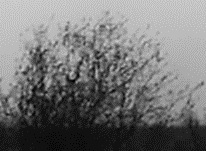
\includegraphics[scale=0.5]{imagenes/ImgsSplinesBloquesFijos/lagok1525.jpg}
}
\subfloat[2, 200]{
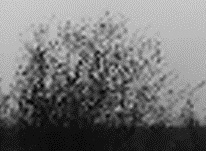
\includegraphics[scale=0.5]{imagenes/ImgsSplinesBloquesFijos/lagok2200.jpg}
}
\subfloat[3, 100]{
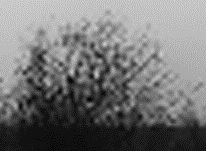
\includegraphics[scale=0.5]{imagenes/ImgsSplinesBloquesFijos/lagok3100.jpg}
}
\subfloat[5, 50]{
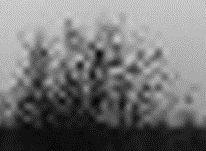
\includegraphics[scale=0.5]{imagenes/ImgsSplinesBloquesFijos/lagok550.jpg}
}
\subfloat[7, 382]{
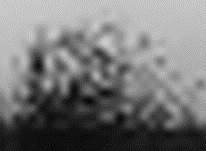
\includegraphics[scale=0.5]{imagenes/ImgsSplinesBloquesFijos/lagok7382.jpg}
}
\caption{Comparación entre la imagen original y la procesada con distintos $k$. Debajo de cada imagen se encuentra su respectivo $k$ y tamaño de bloque utilizado.}
\end{figure}
\noindent Dado que probamos el método con varios valores de $k$ y varios tamaños de bloque, para presentar mejor la información usaremos una tabla por cada valor de $k$: 
\newline

\centerline{
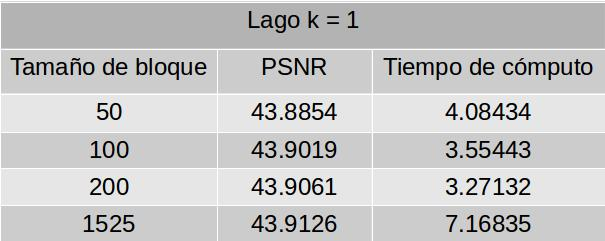
\includegraphics[scale=0.5]{imagenes/lagok1Tabla.jpg}
}
\vspace{1cm}

\centerline{
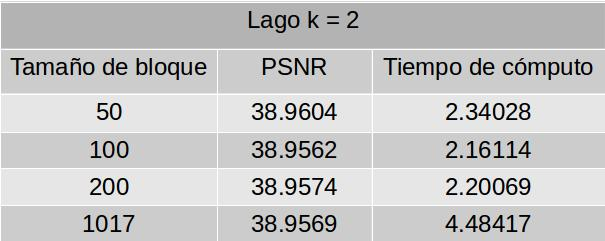
\includegraphics[scale=0.5]{imagenes/lagok2Tabla.jpg}
}
\vspace{1cm}

\centerline{
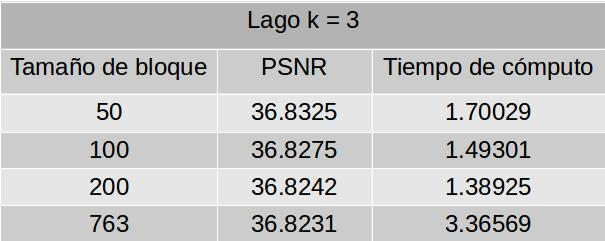
\includegraphics[scale=0.5]{imagenes/lagok3Tabla.jpg}
}
\vspace{1cm}

\centerline{
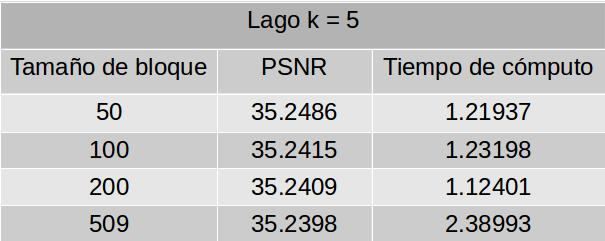
\includegraphics[scale=0.5]{imagenes/lagok5Tabla.jpg}
}
\vspace{1cm}

\centerline{
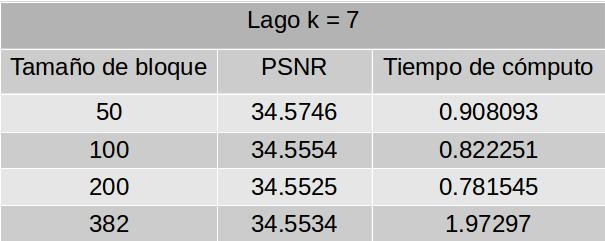
\includegraphics[scale=0.5]{imagenes/lagok7Tabla.jpg}
}
En todas las tablas se cumple que el tiempo de cómputo correspondiente a procesar la imagen con un solo bloque grande, es mayor que utilizando bloques de tamaños más pequeños. Esta diferencia se acentúa cuando la imagen de la cual partimos es más grande y, a medida que vamos tomando $k$ mayores la diferencia se va haciendo más chica. En conclusión, la diferencia es notoria, lo que sucede es que cuando trabajamos con imágenes chicas el tiempo de cómputo ya de por sí es chico y es por eso que tanto trabajar con un bloque grande como trabajar con bloques chicos va a demandar un costo computacional bajo. También podemos ver que esta diferencia es relevante cuando la diferencia del tamaño de bloque es necesariamente grande ya que para los tamaños 50, 100 y 200 que utilizamos, en $k = 1, 3$ y $7$ nos dió un tiempo de cómputo mayor para 50 que para 100 y mayor para 100 que para 200.
\par En cuanto a los PSNR observados, no se puede concluir nada sobre si es mejor utilizar un tamaño de bloque u otro ya que son todos muy similares y, por ejemplo si miramos para $k = 1$, se registra un aumento a medida que aumenta el tamaño de bloque pero para $k = 3, 5, 7$ pasa exactamente lo contrario. $k = 2$ es el caso que nos incita a pensar que, para este tipo de imágenes, poco influye en el PSNR un tamaño de bloque u otro, ya que a diferencia de los demás $k$, no hay un crecimiento o decrecimiento estricto del PSNR según el tamaño del bloque.


Pasemos ahora a analizar la imagen Piano. Este es otro ejemplo para el cuál visualmente el método funciona muy bien. Las diferencias entre imágenes procesadas con distintos tamaños de bloque son, al igual que en el caso anterior, imperceptibles. Además de que, la única diferencia realmente notoria entre la imagen original y las resultantes, es el borde de las teclas negras (sobre todo de la tercera), el cual se despixelea un poco.

\begin{figure}[H]
\centering
\subfloat[Original]{
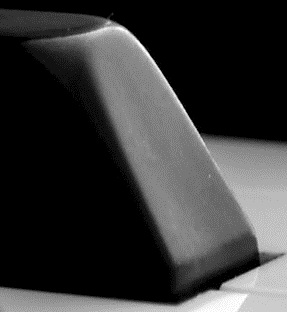
\includegraphics[scale=0.5]{imagenes/ImgsSplinesBloquesFijos/pianooriginal.jpg}
}
\subfloat[1, 775]{
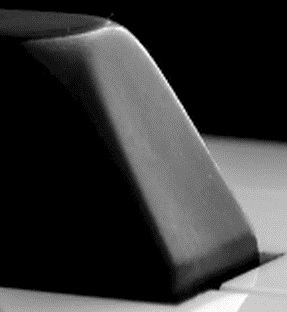
\includegraphics[scale=0.5]{imagenes/ImgsSplinesBloquesFijos/pianok1775.jpg}
}
\subfloat[2, 100]{
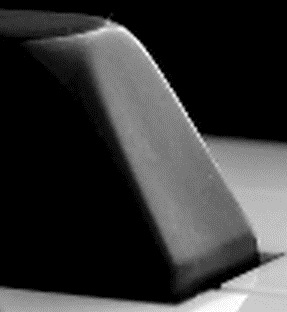
\includegraphics[scale=0.5]{imagenes/ImgsSplinesBloquesFijos/pianok2100.jpg}
}
\subfloat[3, 388]{
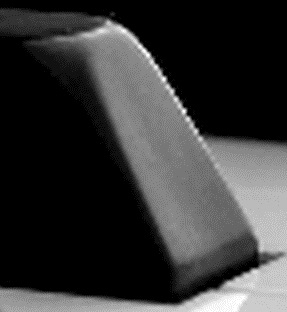
\includegraphics[scale=0.5]{imagenes/ImgsSplinesBloquesFijos/pianok3388.jpg}
}
\caption{Comparación entre la imagen original y la procesada con distintos $k$. Debajo de cada imagen se encuentra su respectivo $k$ y tamaño de bloque utilizado.}
\end{figure}

Esta diferencia aumenta con el $k$. Una posible razón por la cual sucede esto es por la iluminación que tiene la imagen, el borde de la tercera tecla negra esta bien definido en la imagen original pero al ser blanco por el reflejo de la luz y tener de un lado negro y del otro gris, como el spline va a tener en cuenta toda esta información se va a terminar mezclando de alguna manera y al estar bien definido va a resultar notorio. Es por eso que no pasa tanto con las otras teclas donde el borde es más difuso. La tabla para esta imagen es la siguiente:
\newline

\centerline{
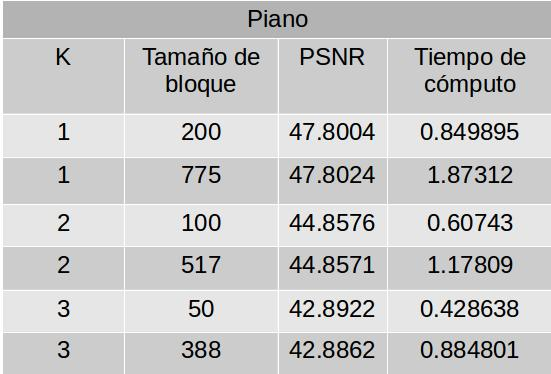
\includegraphics[scale=0.5]{imagenes/pianoTabla.jpg}
}


Como podemos ver, no queda claro aca tampoco cuál es el tamaño de bloque a utilizar ya que, dependiendo el $k$ a veces tomar un tamaño de bloque relativamente mediano (en comparación al tamaño de la imagen) da mejor que procesar la imagen como un solo bloque mientras otras veces pasa lo contrario. En relación al tiempo de cómputo, se mantiene nuestra teoría de que procesando la imagen con un solo bloque grande es más costoso que con muchos de tamaño menor por la cantidad de información necesaria para construir cada spline.


Analicemos ahora la imagen Rosa. Vamos a estar trabajando con un tamaño de bloque bastante chico en relación al tamaño de la imagen, debido a que ésta contiene numerosos detalles y por lo tanto de un bloque a otro puede cambiar significativamente. Los $k$ van a ser 1, 2 y 5. En este caso nuevamente las diferencias entre imágenes procesadas con un tamaño de bloque u otro no son relevantes. En cuanto a las diferencia con la imagen original, éstas son realmente apreciables recién para $k = 5$, entre ellas podemos encontrar la forma de algunas gotas y, en mayor medida, los bordes. El despixelado que se produce en los bordes es notable por el mismo motivo que en la imagen Piano, al tener gotas que tienen una tonalidad más clara que los borde, sombras que son mucho más oscuras o mismo el reflejo de la luz, se mezclan los tonos y, cuando el borde está bien definido se genera el despixelado.

\begin{figure}[H]
\centering
\subfloat[Original]{
\includegraphics[scale=0.5]{imagenes/ImgsSplinesBloquesFijos/rosaoriginal.jpg}
}
\subfloat[1, 1024]{
\includegraphics[scale=0.5]{imagenes/ImgsSplinesBloquesFijos/rosak11024.jpg}
}
\subfloat[2, 683]{
\includegraphics[scale=0.5]{imagenes/ImgsSplinesBloquesFijos/rosak2683.jpg}
}
\subfloat[5, 342]{
\includegraphics[scale=0.5]{imagenes/ImgsSplinesBloquesFijos/rosak5342.jpg}
}
\caption{Comparación entre la imagen original y la procesada con distintos $k$. Debajo de cada imagen se encuentra su respectivo $k$ y tamaño de bloque utilizado.}
\end{figure}

Si observamos la imagen completa, podemos ver que en los bordes de la parte inferior izquierda no se produce despixelado o por lo menos no se puede ver, porque ya vienen difusos. La tabla para esta imagen es la siguiente:
\newline

\centerline{
\includegraphics[scale=0.5]{imagenes/rosaTabla.jpg}
}

Al parecer nuestra hipótesis de que el método podía funcionar mejor tomando la imagen de a pequeños bloques por tener muchos detalles, no era cierta. Esto se ve en los números dado que para los tres valores de $k$ utilizados, obtenemos un PSNR mayor cuando procesamos la imagen con un solo bloque del tamaño de la misma. También se probó con valores de tamaño de bloque mucho más reducidos como 5x5 y aún así seguía dando mayor PSNR procesando la imagen con un solo bloque, aunque al igual que sucede con estos resultados, las diferencias de PSNR no fueron demasiado grandes.


Finalmente analizamos nuestra última imagen para Splines: Auto. Dado que el tamaño de esta imagen es el más grande, vamos a trabajar con más valores de $k$, que serán los siguientes: 2, 4, 6, 8 y 12. Dado que esta imagen tiene muchísimos detalles y, considerando los resultados obtenidos con la imagen Rosa, esta vez decidimos tomar un tamaño de bloque más. De esta manera apuntamos a tener un tamaño chico, otro mediano-grande y el que siempre usamos del tamaño de la imagen, para poder ver si vuelve a suceder que gana el tamaño del bloque mayor o fue un resultado particular de la imagen anterior.	 Los tamaños de los bloques los vamos a mostrar explicitamente cuando veamos la tabla ya que varían según el $k$.

\begin{figure}[H]
\centering
\subfloat[Original]{
\includegraphics[scale=0.5]{imagenes/ImgsSplinesBloquesFijos/autooriginal.jpg}
}
\subfloat[4, 820]{
\includegraphics[scale=0.5]{imagenes/ImgsSplinesBloquesFijos/autok4820.jpg}
}
\subfloat[6, 30]{
\includegraphics[scale=0.5]{imagenes/ImgsSplinesBloquesFijos/autok630.jpg}
}
\subfloat[8, 456]{
\includegraphics[scale=0.5]{imagenes/ImgsSplinesBloquesFijos/autok8456.jpg}
}
\subfloat[12, 10]{
\includegraphics[scale=0.5]{imagenes/ImgsSplinesBloquesFijos/autok1210.jpg}
}
\caption{Comparación entre la imagen original y la procesada con distintos $k$. Debajo de cada imagen se encuentra su respectivo $k$ y tamaño de bloque utilizado.}
\end{figure}

\par Una vez más, sucede que las diferencias entre las imágenes procesadas tanto con bloques chicos como medianos y un único bloque se llegan a apreciar bien recién para $k = 12$. Las diferencias con la imagen original hasta $k = 6$ se notan más que nada en las lineas claras que representan los reflejos, las cuales se empiezan a segmentar de alguna manera, alternando con el color oscuro del auto. Para $k = 8$ y $k = 12$ ya podemos ver que los bordes se empiezan a despixelar bastante, es fácilmente apreciable en los del parabrisas (sobre todo en el que está sobre el reflejo de la luz y hace que se mezcle la parte clara con la oscura) y en las letras del logo.
\noindent \newline Para poder ver si efectivamente sucede lo mismo que con la imagen Rosa, con respecto a los bloques y el PSNR, a continuación mostramos las tablas correspondientes a esta imagen:
\newline

\centerline{
\includegraphics[scale=0.5]{imagenes/autok2Tabla.jpg}
}
\vspace{1cm}

\centerline{
\includegraphics[scale=0.5]{imagenes/autok4Tabla.jpg}
}
\vspace{1cm}

\centerline{
\includegraphics[scale=0.5]{imagenes/autok6Tabla.jpg}
}
\vspace{1cm}

\centerline{
\includegraphics[scale=0.5]{imagenes/autok8Tabla.jpg}
}
\vspace{1cm}

\centerline{
\includegraphics[scale=0.5]{imagenes/autok12Tabla.jpg}
}

Al igual que sucedió con la imagen Rosa, fueron pocos los casos en donde tomar bloques de tamaño pequeño significó una mejor en el PSNR, exactamente sucedió en $k = 2, 6$. Las diferencias entre el tiempo de cómputo procesando la imagen con un bloque grande y procesándola con muchos de tamaño menor sigue siendo significativa y creciente cuando disminuye el $k$.
\par Como conclusión de toda esta extensa experimentación, podemos decir que cuando tenemos una imagen que podemos dividir en bloques cuadrados de igual tamaño (como lo fue Cuadrícula), conviene utilizar bloques precisamente de ese tamaño. Ahora bien si nuestra imagen es grande y sabemos poco sobre ella, a nivel PSNR da lo mismo si utilizamos muchos bloques o un bloque grande para procesarla, sin embargo es preferible utilizar bloques relativamente chicos porque, según lo observado en la experimentación, el tiempo de cómputo va a ser menor. En resumen, utilizar bloques de tamaño chico parece ser la mejor alternativa.


\subsection{Tiempo de computo}

Luego de hacer pruebas con distintas imágenes nos dimos cuenta que el tiempo de computo de cada método depende solo de la cantidad de pixeles de la imágen en cuestión, lo cual es esperable ya que los algoritmos desarrollados no tienen saltos condicionales según el contenido de los pixeles. En la figura~\ref{tiempoComputo} encontramos una comparación entre el tiempo de computo de cada método según la cantidad de pixeles de la imágen.

\label{tiempoComputo}

Podemos ver que uno es mas rapido que el otro, sin embargo el otro tiene mas calidad

\subsection{Spline 2:}

Para comparar la performance cualitativa así como el tiempo de computo, de aplicar esta variante al método anterior, se trabajaran con las mismas imágenes que utilizo el mismo. Como la cantidad de puntos que se van a utilizar para conformar un spline, tamaño del bloque, ahora está ligado a la tolerancia de diferencia con que se trabaje, $\alpha$. Experimentaremos con distintos valores para cada imagen, empezaremos con una diferencia mínima de 40, aproximadamente una tolerancia del 16\%, e iremos incrementando este valor en 40 hasta una diferencia máxima de 200, 78\%, no optaremos por valores más bajo ya que se asemejaría a aplicar vecino más cercano, ni valores mayores ya que sería similar a utilizar el método anterior tomando como bloque toda la imagen. Además trabajaremos con distintos valores de k por imagen para ver cómo repercute (si es que lo hace).   

Una hipótesis que podemos elaborar es que a mayor k la imagen resultante difiere más de la original, ya que se pierden más datos.    



\begin{figure}[H]
    \centering
    \includegraphics[scale=0.4]{imagenes/tanque1.jpg}
    \caption{Imagen $Tanque$ de 256x256.}
	\label{tanquee}
    \end{figure}
	
\begin{figure}[H]
    \centering
    \includegraphics[scale=0.4]{imagenes/tanque2.jpg}
    \caption{Imagen $Tanque$ de 171x171.}
	\label{tanquee}
    \end{figure}
    
\begin{figure}[H]
    \centering
    \includegraphics[scale=0.4]{imagenes/tanque4.jpg}
    \caption{Imagen $Tanque$ de 103x103.}
	\label{tanquee}
    \end{figure}    
    
La elección de la imagen $Tanque$ estaba ligada a que presenta una uniformidad de color, se puede observar un paisaje con solo un objeto, el tanque, y a la vista la tonalidad del mismo no difiere mucho del fondo. Por lo que la particularidad de este método solo se aplicaría a valores de $\alpha$ bajos, mientras que para los otros la cantidad y los puntos que conforman cada spline serían los mismos. Y esto es lo que se puede observar en la figura \ref{tanquee}, solo el valor $\alpha$ = 40 es el que presenta mayor diferencia entre los distintos alphas. Sin embargo, al utilizar este valor de alpha se obtiene un mayor error, esto se puede deber a que como se trabaja con una diferencia muy baja no es muy restrictiva, por lo que estaría tomando como objetos y/o bordes distintos a partes de las imagen que no lo son y por lo tanto esta replicando valores erróneos. Esto tiene como consecuencia que se presenten una gran cantidad de irregularidades en la misma, algunas de ellas conocidas como artifacts, no solo se perciben en la mayor parte de la imagen si no que se acentúan sobre todo en el tanque, en su contorno, observandose un mayor pixelado en esta sección. 
Otro análisis que se puede hacer a partir de estos valores es que, para k mayores el error aumenta. Esto se debe a que cuando se usan k de mayor valor el tamaño de la imagen a la que se quiere hacer zoom es más pequeña y por lo tanto se tiene menos información. Como consecuencia de estos dos últimos análisis, a simple vista, podemos concluir que para cualquiera de los $\alpha$ se distingue que mientras agrandamos el k la imagen se pixela a un más. Aunque si observamos las imágenes con k = 1 entre sí, no difieren de mucho lo mismo para k = 2, sin embargo para k = 3 recién con los últimos tres valores de $\alpha$ se logra una mejor resolución respecto de ese valor de k. 
        
    
    
    \begin{figure}[H]
    \centering
    \includegraphics[scale=0.4]{imagenes/grises1.jpg}
    \caption{Imagen $Grises$ de 256x256.}
	\label{grisese}
    \end{figure}
    
     \begin{figure}[H]
    \centering
    \includegraphics[scale=0.4]{imagenes/grises2.jpg}
    \caption{Imagen $Grises$ de 171x171.}
	\label{grisese}
    \end{figure}
    
     \begin{figure}[H]
    \centering
    \includegraphics[scale=0.4]{imagenes/grises4.jpg}
    \caption{Imagen $Grises$ de 103x103.}
	\label{grisese}
    \end{figure}
    
    
Al igual que para la imagen anterior corroboramos que el ECM aumenta a medida que lo hace el k, sin embargo en esta caso no aumenta tanto comparados como por ejemplo para las figuras anteriores. Esto podría deberse al tipo de imagen con que ahora trabajamos, la cual son bloques de distintas tonalidades de gris donde no hay muchos detalles que se puedan perder. Algo que a partir de la figura se vuelve a repetir es que para valores de $\alpha$ mayores el ECM disminuye y por lo tanto el PSNR aumenta, originalmente la idea es que la particularidad de este método (hasta donde tomar el spline y que hacer entre el final de un spline y el comienzo del siguiente) debe ser aplicado cuando hay grandes cambios ahora podemos empezar a deducir el valor de esta diferencia. Aún más, empezamos a notar que esta variación tiene graves consecuencias cuando se impone una condición menos restrictiva  obteniendo un mayor error cuadrático. En cuanto a lo que se puede analizar al observar las imágenes resultantes estas no poseen una gran diferencia cuando se las observa, para k= 4 se pueden observar imágenes más ruidosas respecto de los otros k, pero en cuanto a comparar con los $\alpha$ las diferencias entre estos son casi imperceptibles.              
    

\begin{figure}[H]
    \centering
    \includegraphics[scale=0.4]{imagenes/cua1.jpg}
    \caption{Imagen $Cuadricula$ de 256x256.}
	\label{cuade1}
    \end{figure}
    
\begin{figure}[H]
    \centering
    \includegraphics[scale=0.4]{imagenes/cua2.jpg}
    \caption{Imagen $Cuadricula$ de 171x171.}
	\label{cuade2}
    \end{figure}
    
    \begin{figure}[H]
    \centering
    \includegraphics[scale=0.4]{imagenes/cua4.jpg}
    \caption{Imagen $Cuadricula$ de 103x103.}
	\label{cuade3}
    \end{figure}
    
La imagen $Cuadricula$ posee un nivel de detalle mayor que las imágenes anteriores, en esta se observan una gran cantidad de líneas de color negro en un fondo blanco, y en algunas partes estas están muy próximas.
 Si reducimos mucho la imagen los detalles se podrían perder más fácilmente, aumentando el ECM. Cuando observamos los valores arrojados por la figuras \ref{cuade1}, \ref{cuade1}, \ref{cuade1} vemos que esto sucede, es más el error se incrementa en un rango no despreciable mientras que para los distintos valores de  $\alpha$ obtenemos los mismos resultados. Al analizar esto, junto con lo que observamos en las imágenes obtenidas, podemos estableces que como solo interviene dos colores, el blanco y el negro, con valores 0 y 255 respectivamente, siempre vamos a caer en el caso de que un mismo spline no se utilice para toda una fila sino hasta cierto punto, sin importar el valor de $\alpha$.
 En esta imagen es en las que más se puede apreciar como actúa la variación respecto al método original. En las imágenes obtenidas con  k = 1, se notan que las líneas tienen más grosor, esto es acción de la replicación de los valores que establece la idea de vecino más cercano. Para las imágenes obtenidas con los restantes k también se observa esto pero la imagen resultante difiere y por mucho de la original (la mayoría de las trazas de color negro se perdieron y fueron irrecuperables por el método). A su vez trabajar con esta figura nos plantea un nuevo posible experimento a analizar, dado que es evidente la parte en la que actúa vecino más cercano e incluso llega a alterar la imagen, se podrían optar por aplicar otros métodos entre un spline o el otro.

        
    \begin{figure}[H]
    \centering
    \includegraphics[scale=0.4]{imagenes/piano1.jpg}
    \caption{Imagen $Piano1$ de 775x775.}
	\label{piano1}
    \end{figure}
    
    
    \begin{figure}[H]
    \centering
    \includegraphics[scale=0.4]{imagenes/piano2.jpg}
    \caption{Imagen $Piano2$ de 517x517.}
	\label{piano2}
    \end{figure}
    
     \begin{figure}[H]
    \centering
    \includegraphics[scale=0.4]{imagenes/piano3.jpg}
    \caption{Imagen $Piano3$ de 388x388.}
	\label{piano3}
    \end{figure}
    
Una de las particularidades de $Piano$ era observar cómo se comporta nuestro método frente a imágenes que tenían algún tipo de efecto, en este caso reflejos y sobre todo uno tan sutil. Como el reflejo de esta imagen es muy claro, al aumentar el k creeríamos que los puntos a interpolar podrían quedar más claros eliminando dicho efecto. Además deseábamos que se siga manteniendo una clara distinción entre las secciones oscuras que conforman cada tecla respecto de las más claras.
 Si analizamos en cuanto a los valores de las figuras \ref{piano1}, \ref{piano2} y \ref{piano3} observamos que al variar el k, el PSNR disminuye, pero levemente, en este caso como estamos trabajando con una imagen de mayor tamaño pudimos trabajar con varios k sin que se altere demasiado la imagen. Al Fijar un k e ir variando los $\alpha$ las imágenes son muy similares visualmente entre si y respecto de la imagen original. El efecto de reflejo sigue existiendo y visualmente casi sin modificaciones, lo que nos lleva a pensar que el método de spline es útil aun para imágenes con estos detalles. En lo que respecta a las diferencias entre las secciones de las teclas, estas siguen manteniendo sus bordes bien delimitados. 
En este tipo de imágenes donde la cantidad de valores distintos no se limita a una sola franja como en $Cuadricula$, sino que se encuentran en mayor cantidad, el método parece funcionar sin alteraciones visibles. En cambio sí fijamos un valor de alpha y variamos el k entonces se pueden observar algunos artifacts en los bordes de cada tecla, aunque en menor cantidad respecto de las anteriores imágenes.  
    
    \begin{figure}[H]
    \centering
    \includegraphics[scale=0.4]{imagenes/rosa1.jpg}
    \caption{Imagen $Rosa$ de 1024x1024.}
	\label{rosa1}
    \end{figure}
    
    \begin{figure}[H]
    \centering
    \includegraphics[scale=0.4]{imagenes/rosa2.jpg}
    \caption{Imagen $Rosa$ de 683x683.}
	\label{rosa2}
    \end{figure}
    
    \begin{figure}[H]
    \centering
    \includegraphics[scale=0.4]{imagenes/rosa5.jpg}
    \caption{Imagen $Rosa$ de 342x342.}
	\label{rosa3}
    \end{figure}    
    
La imagen $Rosa$ presenta tonalidades de grises similares, por lo que creíamos que no se iba a ver muy alterada al variar el k o el valor de alpha. Sin embargo como se observa en las figuras \ref{rosa1}, \ref{rosa1} y  \ref{rosa1}. Los valores difieren bastante entre cada k usada y alphas empleados. Las mayores diferencias visuales que encontramos, y que pueden ser las causantes de obtener estos valores, son entre las gotas de agua en la rosa. Estos últimos detalles son de una tonalidad opuesta al fondo en donde se encuentran y al ser de muy pequeño tamaño es mas dificultoso trabajar con los mismos. Al utilizar valores de alphas muy bajos, observamos que las gotas en algunos casos aumentan su tamaño, aunque levemente, esto se puede deber a que en esas zonas la variación del método actúa mas frecuentemente y como ya analizamos anteriormente (por ejemplo para la imagen $Cuadricula$) cuando los detalles son de menor tamaño el método no es muy eficaz. Sin embargo, pese a este cambio de tamaño, notamos que las tonalidades de las gotas son muy parecidas a la original, hecho que no ocurre al aumentar alpha. Cuando se aumenta el valor de alpha un mismo spline podría aplicarse tanto en las gotas como en el resto de la rosa, como tiene mas puntos en los que los valores son mayores (por ser tonalidades de grises oscuros) al parecer los bordes de las gotas se ven afectados fuertemente por estos, recién en el centro de las mismas  resultan ser mas claros. 

Para esta imagen pudimos ver que tomas valores de alpha muy grandes  muy pequeños tienen consecuencias notables a la vista.

Como ocurrió en los casos anteriores al aumentar el valor de k la imagen fue perdiendo calidad y casi siempre es evidente entre los bordes de los distintos objetos que componen a una imagen, en este caso entre los pétalos de la rosa donde se evidencia un notable pixelado.\newline  \newline \newline \newline \newline

Las siguientes  dos imágenes fueron utilizadas primordialmente para comparar el tiempo de computo respecto de las anteriores, ya que estas son de mayor dimensión. Además estas nos van a  permite trabajar con una mayor cantidad de k.

    
           \begin{figure}[H]
    \centering
    \includegraphics[scale=0.4]{imagenes/lago1.jpg}
    \caption{Imagen $Lago$ de 1525x1525.}
	\label{lagoe}
    \end{figure}
    
        \begin{figure}[H]
    \centering
    \includegraphics[scale=0.4]{imagenes/lago2.jpg}
    \caption{Imagen $Lago$ de 1017x1017.}
	\label{lagoe}
    \end{figure}
    
        \begin{figure}[H]
    \centering
    \includegraphics[scale=0.4]{imagenes/lago3.jpg}
    \caption{Imagen $Lago$ de 763x763.}
	\label{lagoe}
    \end{figure}
    
    
        \begin{figure}[H]
    \centering
    \includegraphics[scale=0.4]{imagenes/lago5.jpg}
    \caption{Imagen $Lago$ de 509x509.}
	\label{lagoe}
    \end{figure}
    
    
        \begin{figure}[H]
    \centering
    \includegraphics[scale=0.4]{imagenes/lago7.jpg}
    \caption{Imagen $Lago$ de 382x382.}
	\label{lagoe}
    \end{figure}
    
    
Trabajando con mas valores de k, pudimos corroborar que se sigue cumpliendo que al aumentar el valor del mismo, el ECM aumenta y por lo tanto el PSNR disminuye. También observamos que no siempre se incrementa en la misma magnitud, las imágenes en las que existen secciones de tonalidades similares, se siguen manteniendo. En esta imagen aun aumentando el valor de k, las zonas del cielo y del agua permanecían, visiblemente, similares entre si y también con respecto a la imagen origina; no sucedía lo mismo para el sector del terreno donde si empezaron a aparecer artifacts, al igual que en la mayoría de los casos cuando se producían grandes cambios de tonalidad, en este caso entre las distintas superficies del terreno. Los artifacts presentes en esta imagen fueron en los bordes, apareciendo un notable pixelado, mientras que en las secciones mas oscura la imagen fue mucho mas ruidosa. Aún cuando se aumentaba el valor de alpha siendo que en otras imagenes esto a veces perimitia algun tipo de corrección.   
    
    
    
    \begin{figure}[H]
    \centering
    \includegraphics[scale=0.4]{imagenes/auto2.jpg}
    \caption{Imagen $Auto$ de 1366x1366.}
	\label{autoe}
    \end{figure}

    \begin{figure}[H]
    \centering
    \includegraphics[scale=0.4]{imagenes/auto4.jpg}
    \caption{Imagen $Auto$ de 820x820.}
	\label{autoe}
    \end{figure}    
    
    \begin{figure}[H]
    \centering
    \includegraphics[scale=0.4]{imagenes/auto6.jpg}
    \caption{Imagen $Auto$ de 586x586.}
	\label{knnTasa2}
    \end{figure}
    
    
    \begin{figure}[H]
    \centering
    \includegraphics[scale=0.4]{imagenes/auto8.jpg}
    \caption{Imagen $Auto$ de 456x456.}
	\label{knnTasa2}
    \end{figure}
    
    
    \begin{figure}[H]
    \centering
    \includegraphics[scale=0.4]{imagenes/auto12.jpg}
    \caption{Imagen $Auto$ de 316x316.}
	\label{knnTasa2}
    \end{figure}
    
 
Luego de todas las imágenes empleadas podemos deducir que la variación que establecimos, en general, resulta mas eficaz cuando la restricción es menor es decir a valores mayores de alphas. Si alpha es muy chico empieza a distinguir sectores que no son deseados, aunque el tipo de imagen con la que se trabaja influye notablemente. En $auto$ los reflejos y las calcomanías sobre el automóvil comienzan a exagerarse a tal punto de obtener un gran pixelado. Esto último podría deberse a que como en las mayorías de las imágenes al aumentar el valor de k, se pierde mucha información, ya que trabajamos con imágenes mas pequeñas. Sin embargo, en este caso aun para los valores de k mas bajos las imágenes obtenidas varían visualmente mucho respecto de la original y lo hace para los distintos valores alpha similarmente con lo ocurrido para la imagen $Rosa$. Las causas de estas alteración podrían deberse nuevamente a los detalles presentes en la imagen, como ya mencionamos para valores de $\alpha$ muy pequeños comienza comienza a distinguir mas fuertemente distintos sectores de la imagen pero para alpha mayores, en este caso donde los detalles se contraponen fuertemente con el fondo, comienzan a verse influidos por los puntos mas oscuros. 

\subsection{Comparaciones:}
A partir de las experimentaciones realizadas para el método de splines tomando tanto un tamaño fijo del bloque o siendo este variable. Dado que siempre observamos que a mayor PSNR obtenemos visualmente una imagen con mejor calidad y/o similar a la original, procedimos a realizar una tabla comparativa entre los distintos valores de PSNR obtenidos.  

 \begin{figure}[H]
    \centering
    \includegraphics[scale=0.4]{imagenes/tanqueMetodosDif.jpg}
	\label{autoe}
    \end{figure}

 \begin{figure}[H]
    \centering
    \includegraphics[scale=0.4]{imagenes/grisesMetodosDif.jpg}
	\label{autoe}
    \end{figure}
    
    
     \begin{figure}[H]
    \centering
    \includegraphics[scale=0.4]{imagenes/cuadriculaMetodosDif.jpg}
	\label{autoe}
    \end{figure}
    
     \begin{figure}[H]
    \centering
    \includegraphics[scale=0.4]{imagenes/pianoMetodosDif.jpg}
	\label{autoe}
    \end{figure}
    
    
     \begin{figure}[H]
    \centering
    \includegraphics[scale=0.4]{imagenes/rosaMetodosDif.jpg}
	\label{autoe}
    \end{figure}

 \begin{figure}[H]
    \centering
    \includegraphics[scale=0.4]{imagenes/lagoMetodosDif.jpg}
	\label{autoe}
    \end{figure}
    
    
     \begin{figure}[H]
    \centering
    \includegraphics[scale=0.4]{imagenes/autoMetodosDif.jpg}
	\label{autoe}
    \end{figure}

Lo que podemos observar de las comparaciones anteriores es que el método de Splines con bloques fijos obtuvo los mayores valores de PSNR, y por lo tanto las imágenes obtenidas menos diferencias respecto de la original. Este resultado comenzaba a deducirse a lo largo  de la experimentación de Spline 2, cuando observábamos que cuando el valor de $\alpha$ aumentaba obteníamos un PSNR mayor (y como bien mencionamos a medida que el valor de alpha aumenta la variación del método se asemeja al método de spline con bloques de tamaño igual a la imagen). Las causas de este resultado podríamos atribuirlas a la decisión de la variante mas importante introducida, que fue el aplicar la idea de vecino mas cercano entre último punto de un spline y el comienzo del otro. La idea era tratar de mantener los bordes bastantes delimitados, sin embargo esto trajo consecuencias en el resto de la imagen y solo era mas eficaz cuando las diferencias fueron mayor a 200. Una forma de probar obtener mejores resultados (si es que es posible) seria aplicar otro método en vez del de vecino, ya que el mismo es uno de los métodos mas simple (aunque creíamos que esta combinacion podría generar mejores resultados) y podría estar mas susceptible a errores.
En conclusión con los resultados presentes podemos atribuir que para obtener mejores resultados cualitativos el método de spline con bloques de tamaño fijo es superior al de tamaño variable. Sin embargo una dificultad que se nos presenta en el primero método es ¿que tamaño de bloque utilizar? ya que como se puede ver en ~\ref{Splines} los mejores resultados no siempre se obtuvieron para bloques de tamaños similares, en algunos casos el tamaño elegido fue muy bajo y en otro casi el tamaño de la imagen total. Como en algunas imágenes la diferencia es muy notable (por ejemplo para $Cuadricula$), aun tener que buscar entre distintos tamaño del bloque seria mucho mas eficaz (en cuanto a calidad) que aplicando el segundo método evaluando en tan solo $\alpha$ = 200 o algún valor superior (que a partir de los resultados obtenidos creemos que es el mejor valor a tomar). Sin embargo si queremos ponderar el tiempo de computo quizás sea preferible optar por el segundo método donde los tiempos de cómputos en general fueron menores, bastando con una sola ejecución y en general, salvo excepciones, los PSNR no variaron en un amplio rango.   

\subsection{Comparando los 3 metodos}

\begin{table}[H]
\centering
\begin{tabular}{|r|r|r|r|r|r|r|}
\hline
\multicolumn{1}{|c|}{k} & \multicolumn{2}{|c|}{Vecino mas cercano} & \multicolumn{2}{|c|}{Bilineal} & \multicolumn{2}{|c|}{Splines} \\ \hline
  & PSNR & Tiempo & PSNR & Tiempo & PSNR & Tiempo \\ \hline
1 & 0 & 0 & 23.1450 & 0 &  22.6002 & 0 \\ \hline
2 & 0 & 0 & 20.9392 & 0 &  20.2488 & 0 \\ \hline
4 & 0 & 0 & 19.4993 & 0 &  18.8017 & 0 \\ \hline
\end{tabular}
\caption{Tabla de PSNR y tiempo de computo de \texttt{mono.tiff} ejecutadas en las mejores variantes de cada m\'etodo de interpolaci\'on variando el k en 1, 2 y 4.}
\label{}
\end{table}


\begin{table}[H]
\centering
\begin{tabular}{|r|r|r|r|r|r|r|}
\hline
\multicolumn{1}{|c|}{k} & \multicolumn{2}{|c|}{Vecino mas cercano} & \multicolumn{2}{|c|}{Bilineal} & \multicolumn{2}{|c|}{Splines} \\ \hline
  & PSNR & Tiempo & PSNR & Tiempo & PSNR & Tiempo \\ \hline
1 & 0 & 0 & 48.2636 & 0 &  47.8024 & 1.87312 \\ \hline
2 & 0 & 0 & 44.9598 & 0 &  44.8576 & 0.60743 \\ \hline
3 & 0 & 0 & 42.7730 & 0 &  42.8922 & 0.42864 \\ \hline
\end{tabular}
\caption{Tabla de PSNR y tiempo de computo de \texttt{Piano.tiff} ejecutadas en las mejores variantes de cada m\'etodo de interpolaci\'on variando el k en 1, 2 y 3.}
\label{}
\end{table}


\begin{table}[H]
\centering
\begin{tabular}{|r|r|r|r|r|r|r|}
\hline
\multicolumn{1}{|c|}{k} & \multicolumn{2}{|c|}{Vecino mas cercano} & \multicolumn{2}{|c|}{Bilineal} & \multicolumn{2}{|c|}{Splines} \\ \hline
  & PSNR & Tiempo & PSNR & Tiempo & PSNR & Tiempo \\ \hline
1 & 0 & 0 & 43.8323 & 0 &  43.9126 & 7.16835 \\ \hline
3 & 0 & 0 & 37.6747 & 0 &  38.9604 & 2.34028 \\ \hline
5 & 0 & 0 & 36.0974 & 0 &  36.8325 & 1.70029 \\ \hline
\end{tabular}
\caption{Tabla de PSNR y tiempo de computo de \texttt{Lago.tiff} ejecutadas en las mejores variantes de cada m\'etodo de interpolaci\'on variando el k en 1, 3 y 5.}
\label{}
\end{table}


\begin{table}[H]
\centering
\begin{tabular}{|r|r|r|r|r|r|r|}
\hline
\multicolumn{1}{|c|}{k} & \multicolumn{2}{|c|}{Vecino mas cercano} & \multicolumn{2}{|c|}{Bilineal} & \multicolumn{2}{|c|}{Splines} \\ \hline
  & PSNR & Tiempo & PSNR & Tiempo & PSNR & Tiempo \\ \hline
1 & 0 & 0 & 37.7469 & 0 &  38.2394 & 0 \\ \hline
3 & 0 & 0 & 32.1074 & 0 &  31.6412 & 0 \\ \hline
7 & 0 & 0 &  29.0710 & 0 & 28.4955 & 0 \\ \hline
\end{tabular}
\caption{Tabla de PSNR y tiempo de computo de \texttt{venus.tiff} ejecutadas en las mejores variantes de cada m\'etodo de interpolaci\'on variando el k en 1, 3 y 7.}
\label{}
\end{table}




\section{Conclusiones}

\begin{thebibliography}{abbrvnat}
\bibitem{burden} Burden R. L., Faires J.D.- Numerical Analysis
\end{thebibliography}

\end{document}

